W związku  z osobą autora niniejszej historii pozostaje fakt, że rozpoczyna się ona od  jego Ojca -- Benedykta, mimo że nie był najstarszym dzieckiem Edwarda i Eufemii Świerczyńskich, naszych wspólnych dziadków i pradziadków. Jego rodzice i proptoplaści naszego rodu Świerczyńskich pobrali się w Lubecku 15 czerwca 1907~r.

\begin{figure}[!h]
\begin{center}
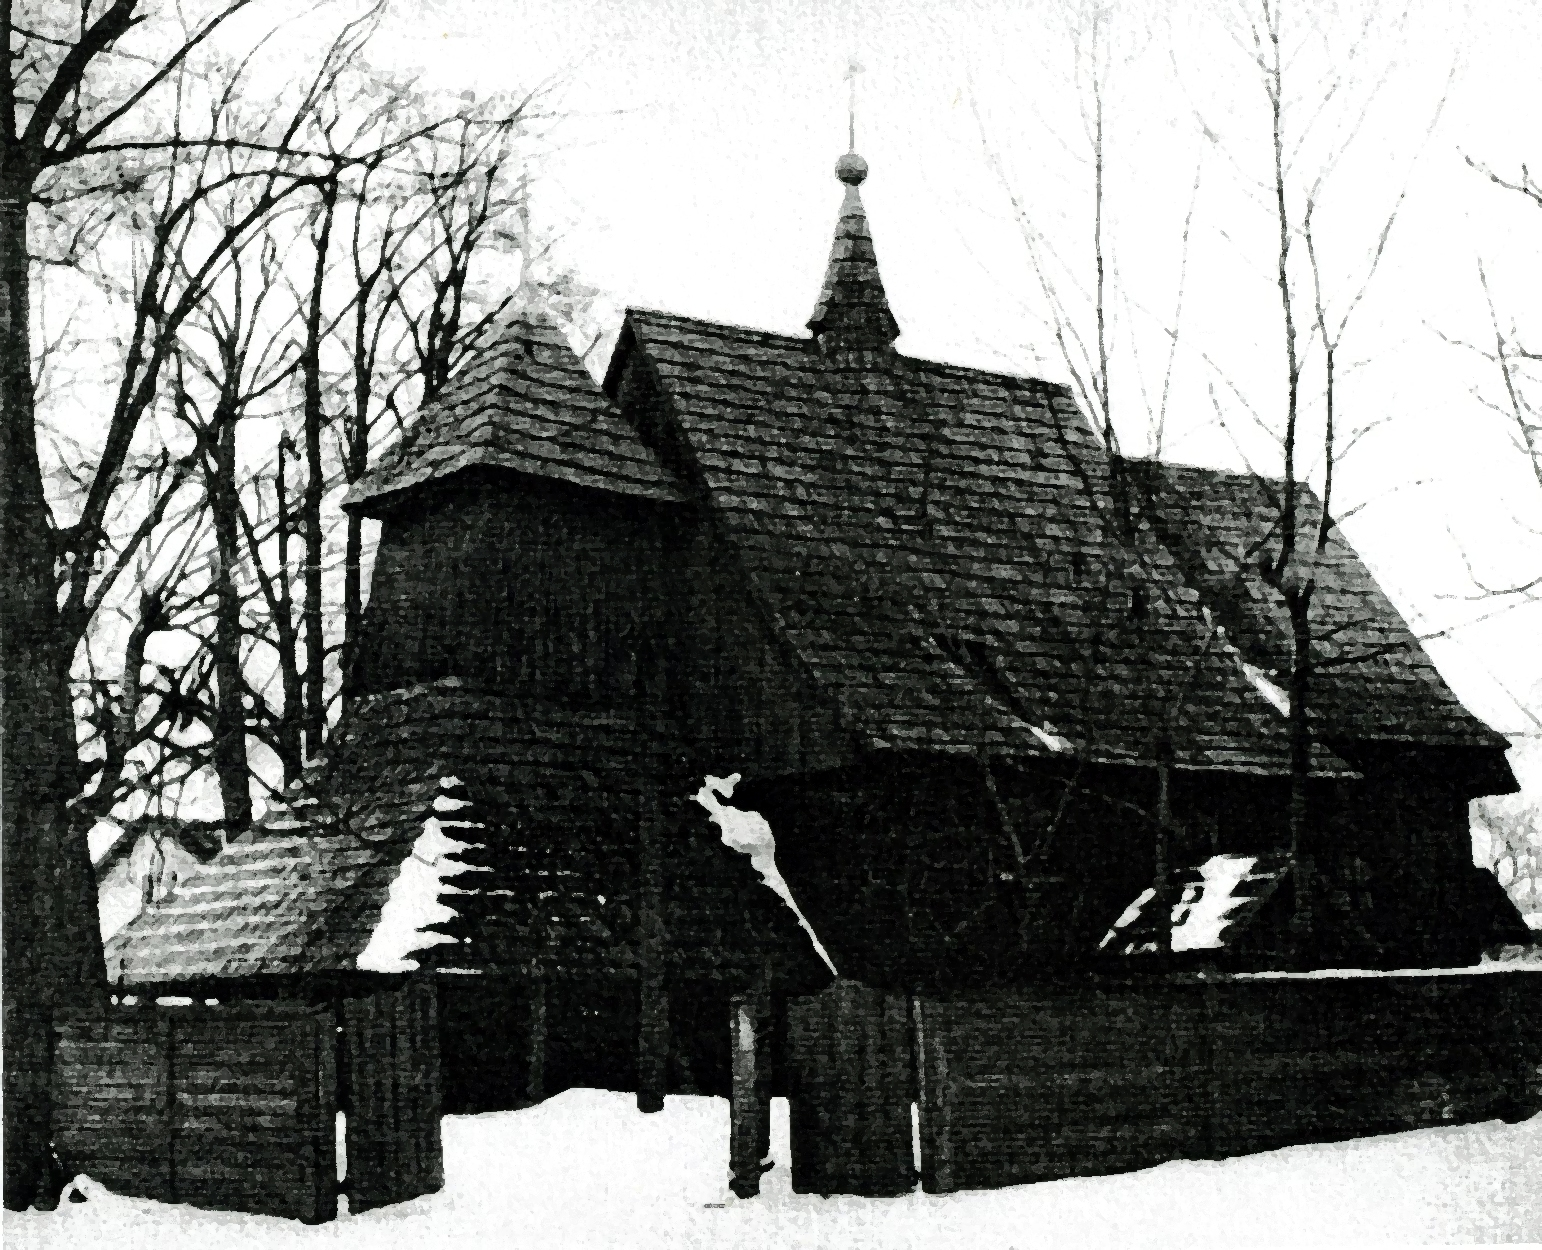
\includegraphics[width=0.6\textwidth]{photo/lagiewniki_wielkie.jpg}
\caption{Stary kościół w Łagiewnikach Wielkich, który spłonął\ldots}
\label{rys:lagiewniki_wielkie}
\end{center}
\end{figure}

\textbf{Benedykt Świerczyński} mój ojciec, a wasz dziadek urodził się w rodzinie małorolnego, ale bardzo ambitnego chłopa dnia \textbf{23 lutego 1920 r.} jeszcze w Rzeszy Niemieckiej, lecz w tej części Górnego Śląska, która wkrótce miała przypaść Polsce.

\begin{figure}[!h]
\begin{center}
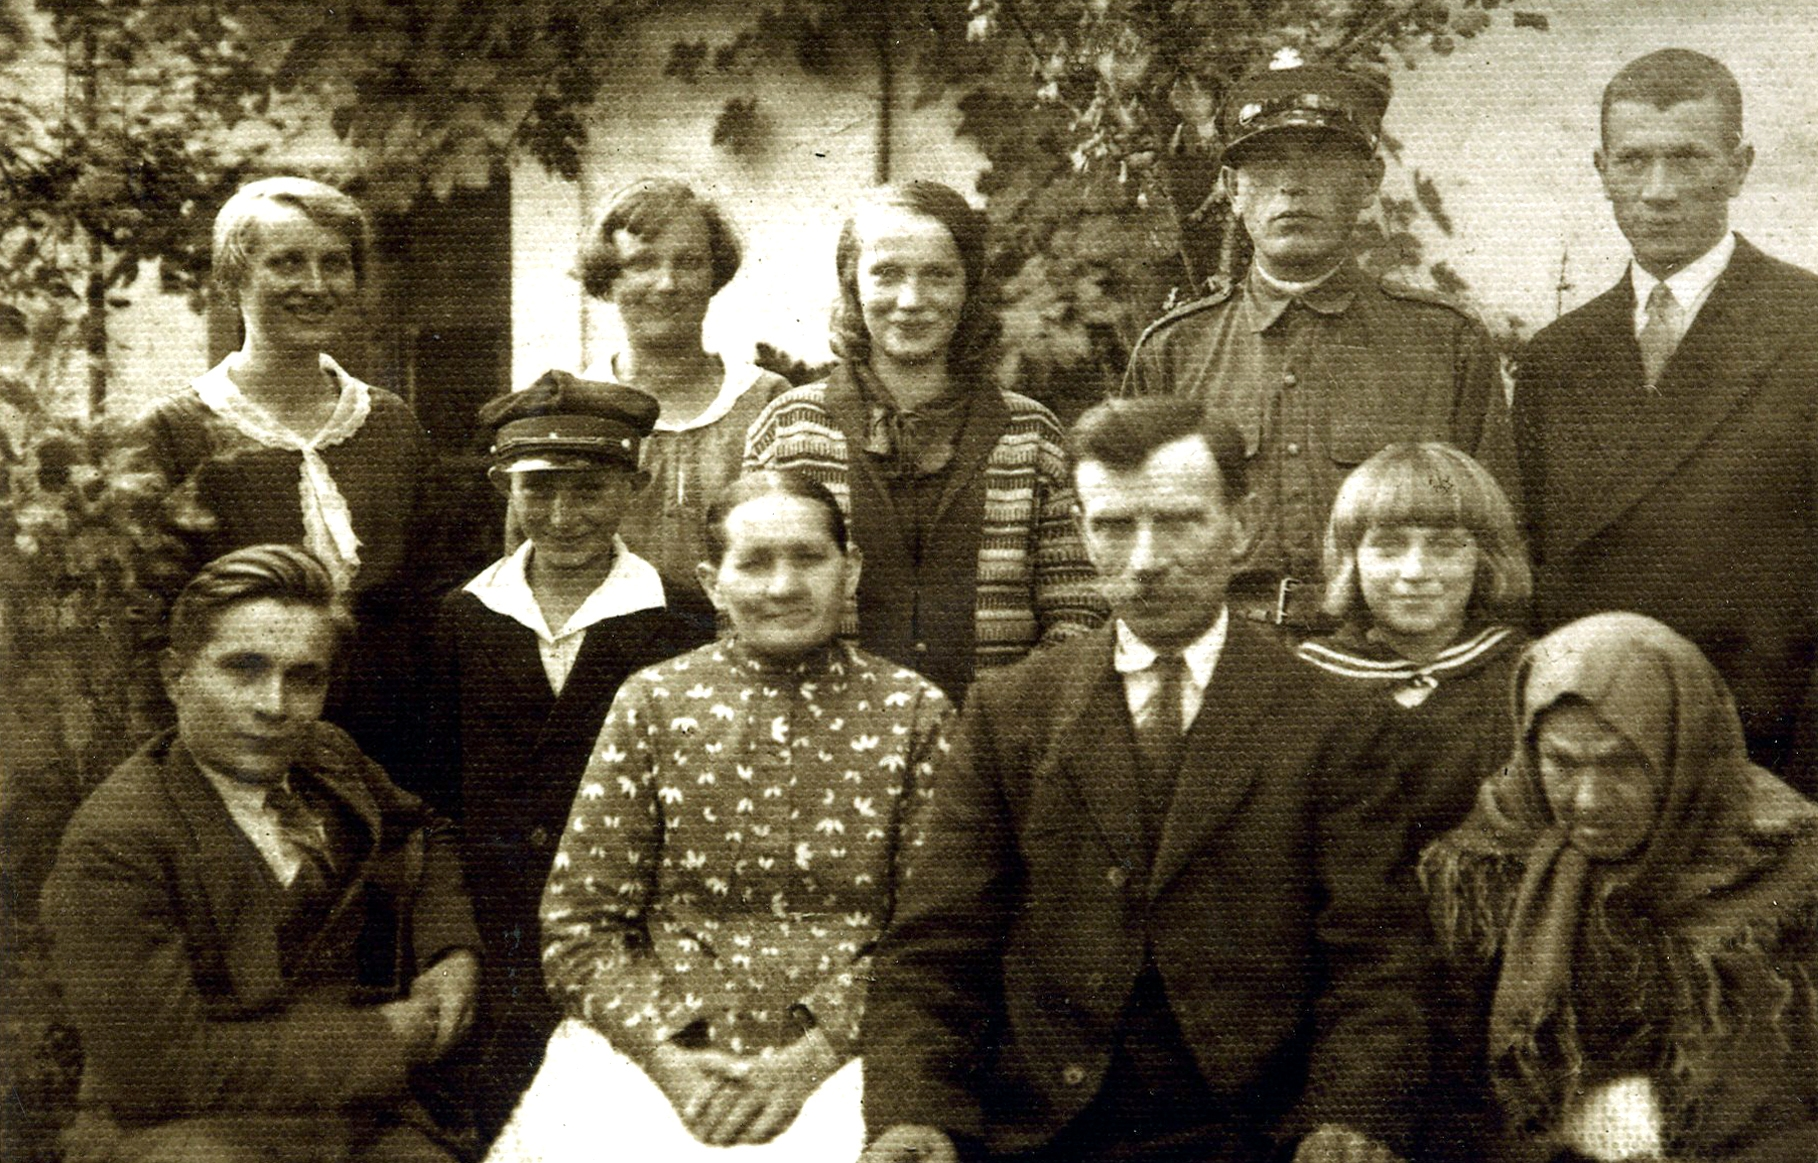
\includegraphics[width=0.6\textwidth]{photo/rodzina_swierczynskich_1.jpg}
\caption[Rodzina Świerczyńskich]{Na zdjęciu rodzina Świerczyńskich: stoją od lewej: Anastazja, Benedykt (w czapce gimnazjalisty), Ludwika (żona Józefa), Irena, Karol i Józef, siedzą Wiktor, babcia Eufemia, dziadek Edward, za nim stoi Rózia, po prawej w chustce siedzi prababcia Julia Świerczyńska z domu Kępa, matka Edwarda.}
\label{rys:rodzina_swierczynskich_1}
\end{center}
\end{figure}

\textbf{Łagiewniki Wielkie}, gdzie się urodził, okazały się miejscowością przygraniczną, w której rogatkach stała komora celna, oddzielająca nie tylko ówczesne Niemcy od Polski, ale też Łagiewniki Wielkie od Ciasna, gdzie mieszkała spora część Świerczyńskich, wywodzących się od Walentego Świerczyńskiego, naszego prapradziadka. Benedykt przyszedł na świat jako szóste dziecko, a czwarty, najmłodszy \textbf{syn Edwarda Świerczyńskiego i Eufemii z domu Grabińskiej}.

Po nim przyszła na świat \textbf{23 lipca 1922 r. Róża Świerczyńska} jako najmłodsze dziecko Edwarda i Eufemii, późniejsza dziedziczka -- wraz ze swym mężem, \textbf{Teodorem Kusiem} -- dóbr ziemskich i zabudowań po naszych dziadkach. Wyszła za niego \textbf{18 listopada 1946 r}.
\begin{figure}[!h]
\begin{center}
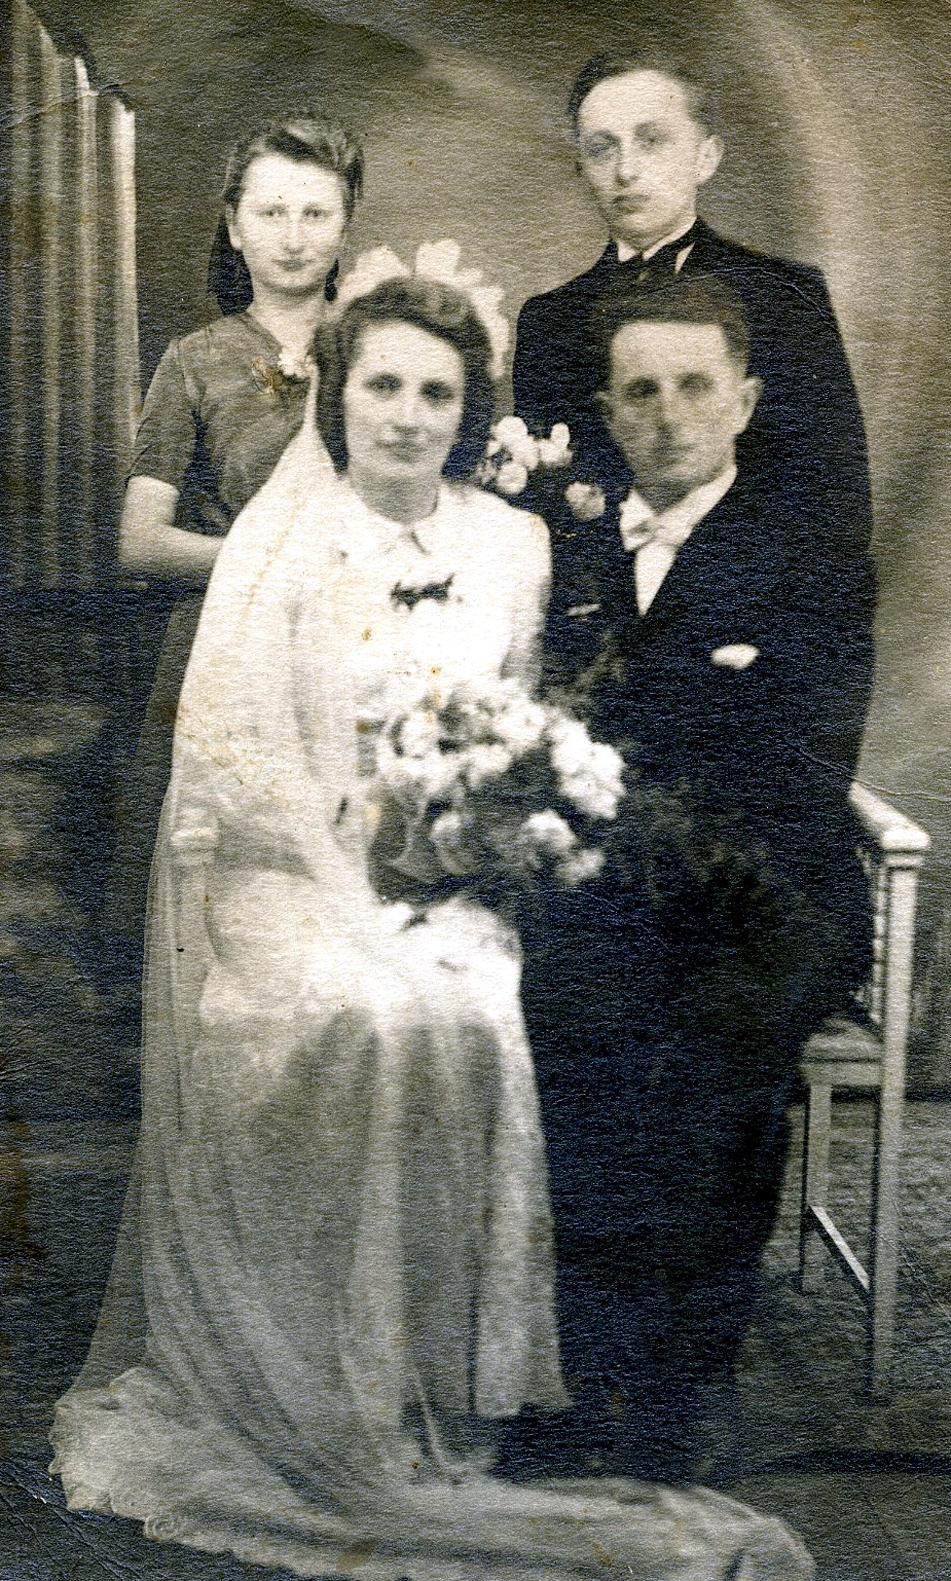
\includegraphics[width=0.36\textwidth]{photo/rozia_teodor_kus_slub.jpg}
\caption[Zdjęcie Ślubne Rózi Świerczyńskiej i Teodora Kusia]{Zdjęcie Ślubne Rózi Świerczyńskiej i Teodora Kusia, stoją za nimi Elżbieta Świerczyńska, córka Józefa i Józef Kuś, brat Teodora.}
\label{rys:rozia_teodor_kus_slub}
\end{center}
\end{figure}

\begin{figure}[!hp]
\begin{center}
\includegraphics[width=0.8\textwidth]{photo/rodzina_kusiow_1.jpg}
\caption[Rodzina Kusiów]{Na zdjęciu siedzą: Bogdan Kuś z synem Adasiem, obok siedzi Krystyna Kuś, za nią Maria Kuś, żona Bogdana, obok Maria Sprycha oraz Irena Lehman. Stoją od dołu: Józef Kuś, wyżej Urszula Świerczyńska (żona Wirgusia) i Lubomira Lehman, nad nią Barbara Walotek, obok solenizantka Rózia Kuś, za nią Katarzyna Kusiówna (c.~Edwarda), za nią na wpół widoczna Klaudia Kuś (c.~Józefa), za nią Zdzisław Walotek (mąż Barbary), obok niego w rogu Agnieszka Ospałek Kuś (żona Artura), za nim Marcin Kuś (s.~Edwarda), za Ireną Lehman stoi agata Walotek (c.~Barbary), za nią Grzegorz Lehman (s.~Lubomiry), za nim Izydor Kuś (s.~Rózi Kuś), za nim Tomasz Lehman (s.~Lubomiry), obok nich Wergiliusz Świerczyński i przy poręczy na wpół widoczny Edward Kuś (s.~Rózi Kuś), poniżej jego żona Regina, obok niej i Grzesia stoi Danka Kuś (c.~Izydora Kusia), po drugiej stronie poręczy stoi Klaudiusz Kuś (s.~Józefa Kusia). Mnie i Tomasza oraz babci Radegundy na tym zdjęciu nie ma, gdyż byliśmy na weselach Zuzi i Aliny Świerczyńskich.}
\label{rys:rodzina_kusiow_1}
\end{center}
\end{figure}



Oczywiście, stryj \textbf{Teodor, syn Franciszka i Elżbiety z domu Malyska} urodzony w Łagiewnikach Wielkich \textbf{18 listopada 1913~r.} wniósł i swoją część, tj. dwa hektary pola na tzw. Gasynce, które kupił za spłatę spadku po rodzicach, którą otrzymał od brata Józefa. Był on szanowanym gospodarzem we wsi oraz wziętym cieślą, który trudnił się zwłaszcza przy stawianiu więźby dachowej. Potrafił iść po kalenicy z ciężką belką na ramieniu. Był silny, odważny i pełen jędrnego chłopskiego humoru, a przy tym zawsze bardzo gościnny. Głos miał silny, donośny. Zresztą na \textbf{Wieskach} -- tak się nazywa ta część Łagiewnik Wielkich -- zawsze godało się głośno i wesoło! Dochowali się pięciorga dzieci: \textbf{Edwarda, Izydora, Marysi, Basi i Bogdana}.
\begin{figure}[!h]
\begin{center}
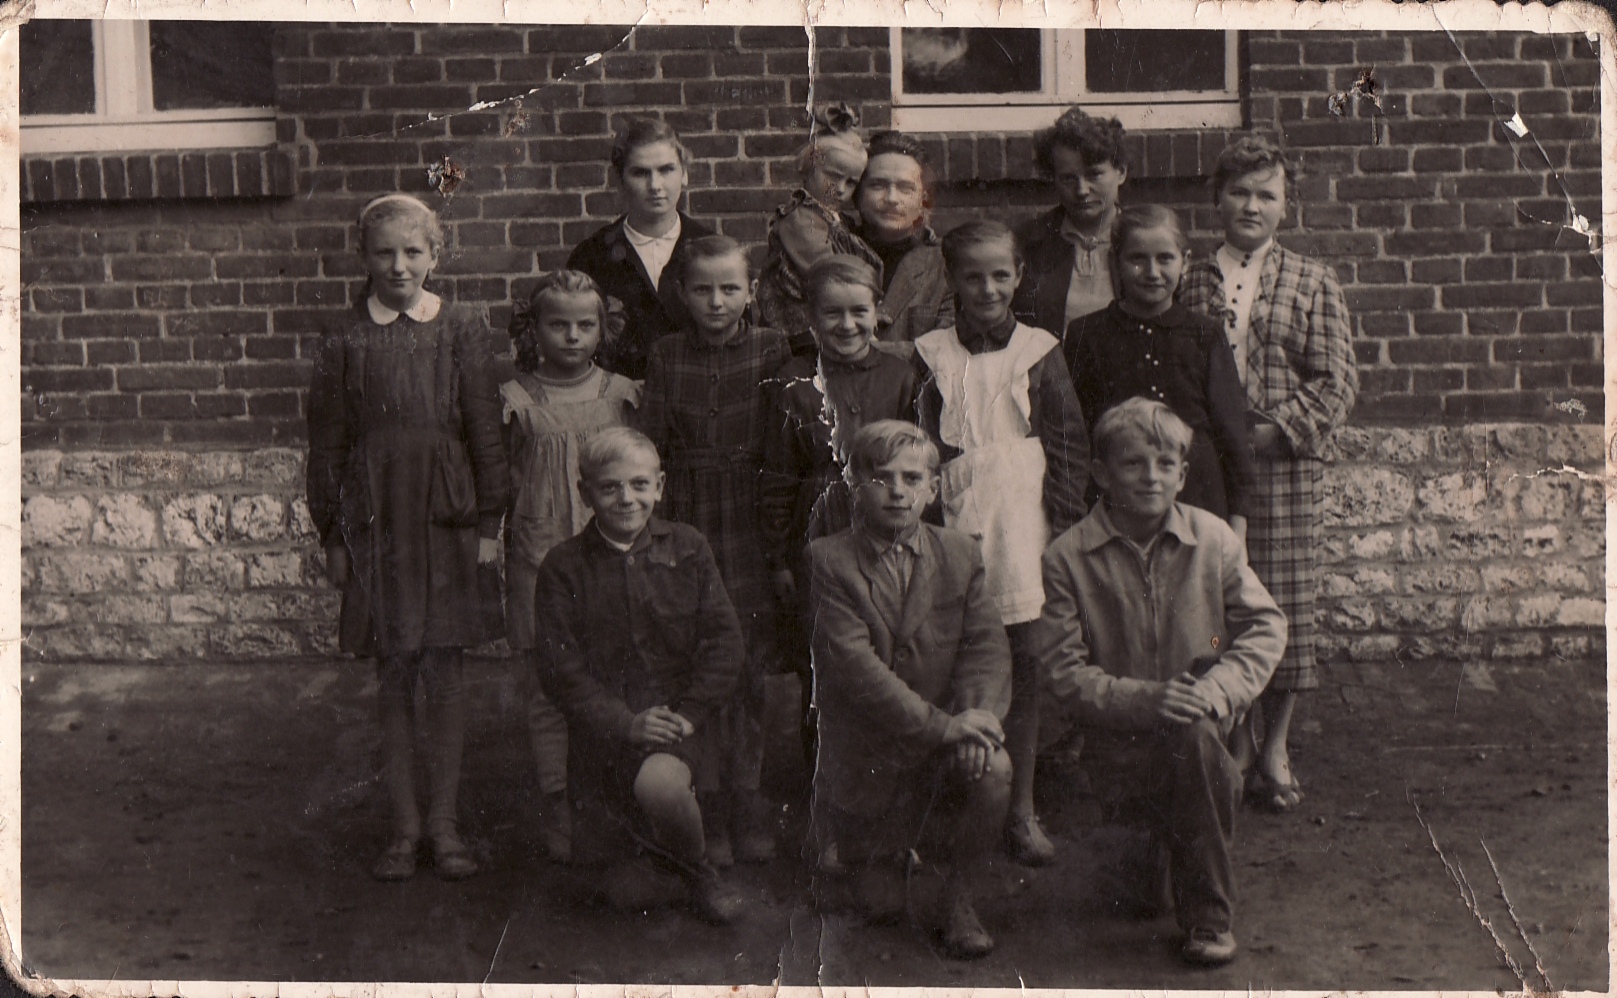
\includegraphics[width=0.6\textwidth]{photo/edward_kus_1.jpg}
\caption[Edward Kuś wśród kolegów, koleżanek i nauczycieli Szkoły Podstawowej w Łagiewnikach Wielkich]{Na zdjęciu Edward Kuś w pierwszym rzędzie pierwszy z prawej wśród kolegów, koleżanek i nauczycieli Szkoły Podstawowej w Łagiewnikach Wielkich.}
\label{rys:edward_kus_1}
\end{center}
\end{figure}

Oboje już nie żyją. \textbf{Teodor zmarł 10 listopada 1996~r.} na parę dni przed szykowanymi już złotymi ich godami... \textbf{Róża zmarła} w dziesięć lat później na raka wątroby \textbf{16~marca 2006~r.} w szpitalu w Zawadzkiem.

Najstarszy ich syn -- \textbf{Edward Kuś,} który wziął imię po dziadku, urodził się \textbf{12 października 1947 r. w Łagiewnikach Wielkich}.

\begin{figure}[!h]
\begin{center}
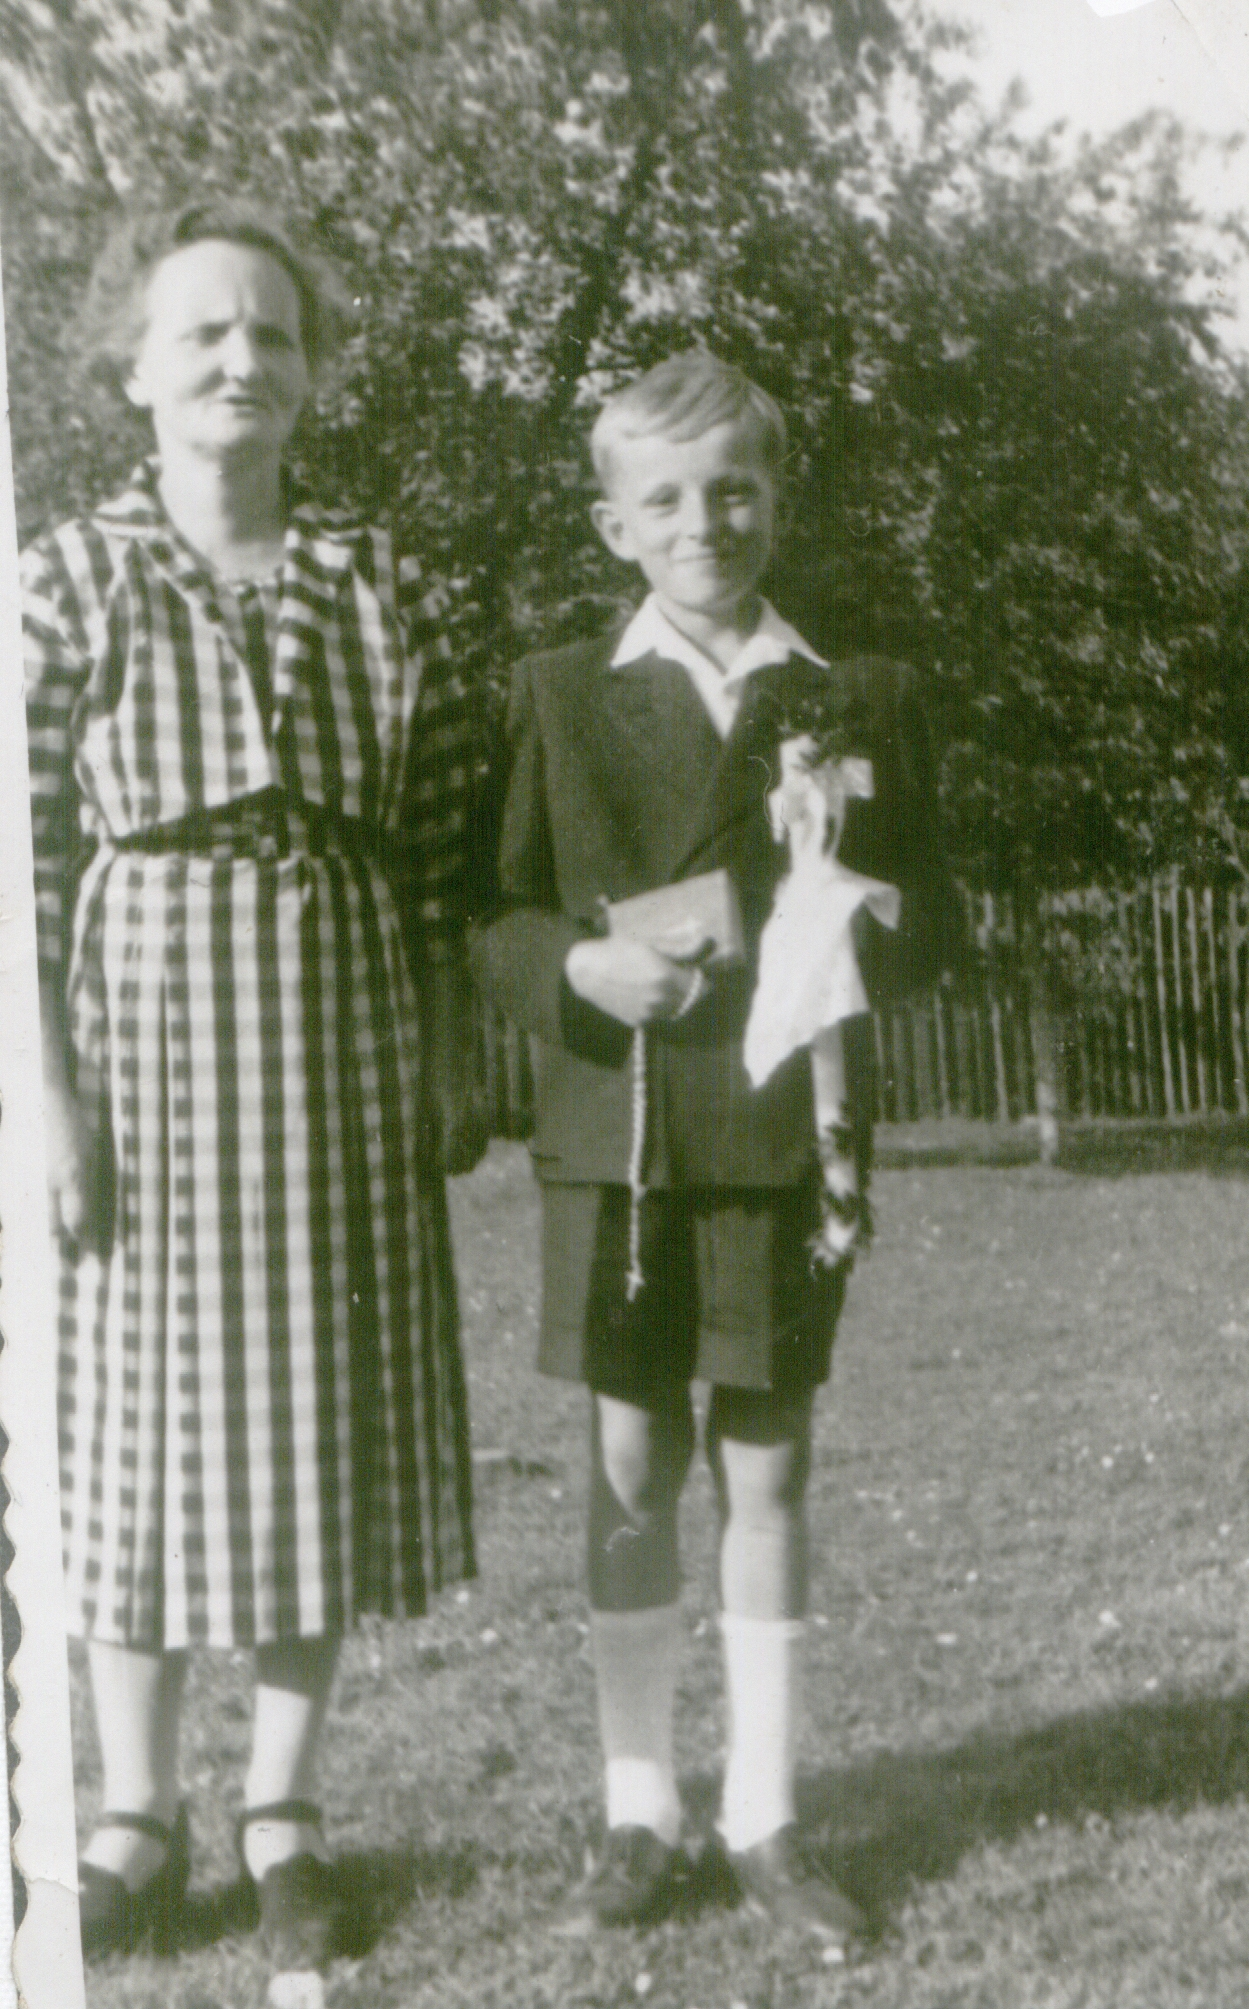
\includegraphics[width=0.32\textwidth]{photo/edward_kus_komunia.jpg}
\caption[Edward Kuś u I Komunii św. ze swoją chrzestną -- ciocią Ludwiką]{Na zdj. Edward Kuś u I Komunii św. stoi ze swoją chrzestną -- ciocią Ludwiką.}
\label{rys:edward_kus_komunia}
\end{center}
\end{figure}

\begin{figure}[!h]
\begin{center}
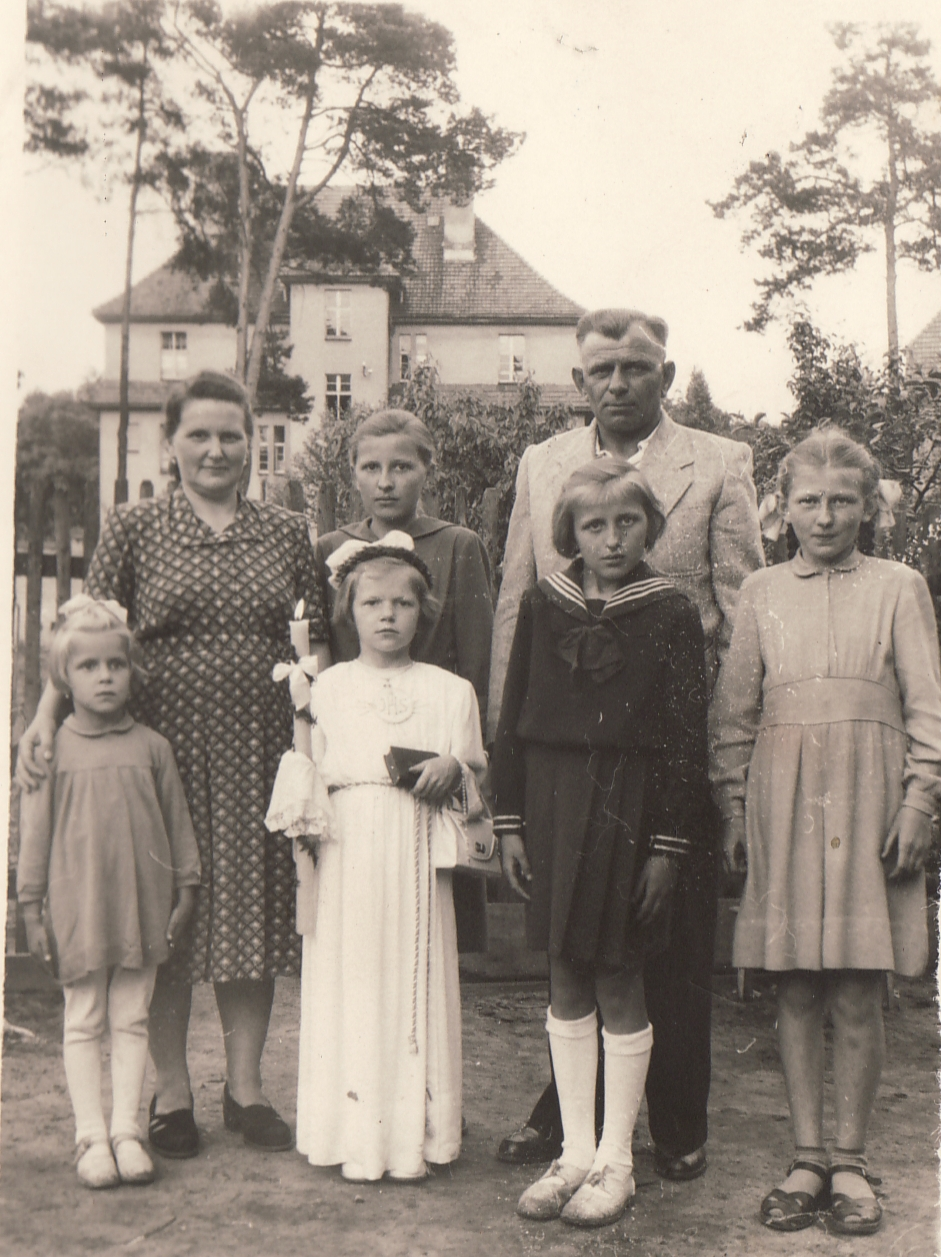
\includegraphics[width=0.4\textwidth]{photo/regina_ruranska_komunia.jpg}
\caption{Pierwsza Komunia św. Reginy Rurańskiej}
\label{rys:regina_ruranska_komunia}
\end{center}
\end{figure}

\begin{figure}[!h]
\begin{center}
\includegraphics[width=0.7\textwidth]{photo/edward_regina_kus_slub.jpg}
\caption[Zdjęcie ślubne Reginy Rurańskiej i Edwarda Kusia]{Zdjęcie ślubne Reginy Rurańskiej i~Edwarda Kusia. Od lewej w~górnym rzędzie: Izydor, Edward i~Bogdan Kusiowie, poniżej Krystyna, żona Izydora, Regina Rurańska Kuś, i~Marysia Kusiówna.}
\label{rys:edward_regina_kus_slub}
\end{center}
\end{figure}

Ukończył Szkołę Zawodową Ślusarską i po odbyciu zasadniczej służby wojskowej zatrudnił się w 1968~r. w Spółdzielni Transportu Wiejskiego jako kierowca samochodów ciężarowych. Uzyskał wszystkie możliwe uprawnienia do kierowania pojazdami mechanicznymi (od kat. A do kat. E). Pracował tam do likwidacji firmy, tj. do 1996~r., w związku z czym przeszedł na przedemerytalny zasiłek, ale dorabiał sobie jako operator koparki. W październiku 2007~r. nabył uprawnienia emerytalne.

\begin{figure}[!h]
\begin{center}
\includegraphics[height=50mm]{photo/edward_regina_kus_dzieci_1.jpg}
\includegraphics[height=50mm]{photo/edward_regina_kus_dzieci_2.jpg}
\includegraphics[height=50mm]{photo/edward_regina_kus_dzieci_3.jpg}
\includegraphics[height=50mm]{photo/marcin_kus_komunia.jpg}
\caption[Dzieci Edwarda i Reginy Kusiów]{Dzieci Edwarda i Reginy Kusiów. Na zdj. 9a Kasia, Artur i Marcin Kuś; na zdj. 9b Edward, Regina,Kasia, Artur (u I Komunii św.), Marcin Kusiowie; na zdj. 9c od lewej Marcin, Artur, Regina, Edward i Katarzyna (u I Komunii św.); na zdj 9d Artur, Marcin (u I Komunii św.) i Katarzyna Kusiowie. }
\label{rys:edward_regina_kus_dzieci_1}
\end{center}
\end{figure}



Jego \textbf{żona Regina, z którą wziął ślub 5 lutego 1972 r. w Lublińcu u o.o. Oblatów, jest córką Józefa Rurańskiego i Gertrudy z domu Kompalla ur. 28 sierpnia 1950 r. w Lublińcu}.

Jako absolwentka Liceum Ogólnokształcącego pracowała w PZGS-ie. Potem, w latach 1982 do 1994 r. przebywała na urlopie macierzyńskim i wychowawczym. Od tego czasu pracuje ona do dzisiaj w kolekturze Totalizatora Sportowego. Mają po rodzicach Reginy dom jednorodzinny w Lublińcu przy ul. Grunwaldzkiej 3. Dochowali się trójki dzieci: \textbf{Artura, Katarzyny i Marcina}.


Ich syn \textbf{Artur urodzony 14 sierpnia 1974~r. w Lublińcu}, ukończywszy technikum mechaniczne podjął pracę w firmie ,,Elfi'' w Lublińcu. Ożenił się z \textbf{Agnieszką z domu Ospałek}, z którą na razie nie ma dzieci.

\textbf{Agnieszka} urodzona \textbf{2~września 1975~r. w Chowaninie z Franciszka i Marii Ospałków} ukończyła technikum ekonomiczne i pracuje w sklepie.

Drugim dzieckiem Edwarda i Reginy Kusiów jest \textbf{Katarzyna urodzona 3 listopada 1975 r. w Lublińcu}, która uzyskawszy tytuł magistra zarządzania i marketingu na Politechnice Gliwickiej, pracuje w Urzędzie Skarbowym w Lublińcu. Wyszła za \textbf{Daniela Rybaka ur. 8 grudnia 1975~r. w Lublińcu z Zygmunta i Aleksandry z domu Mazur} -- nauczyciela wychowania fizycznego w SP w Lisowie i SP w Gwoździanach w gminie Pawonków.

\begin{figure} [!h]
\begin{center}
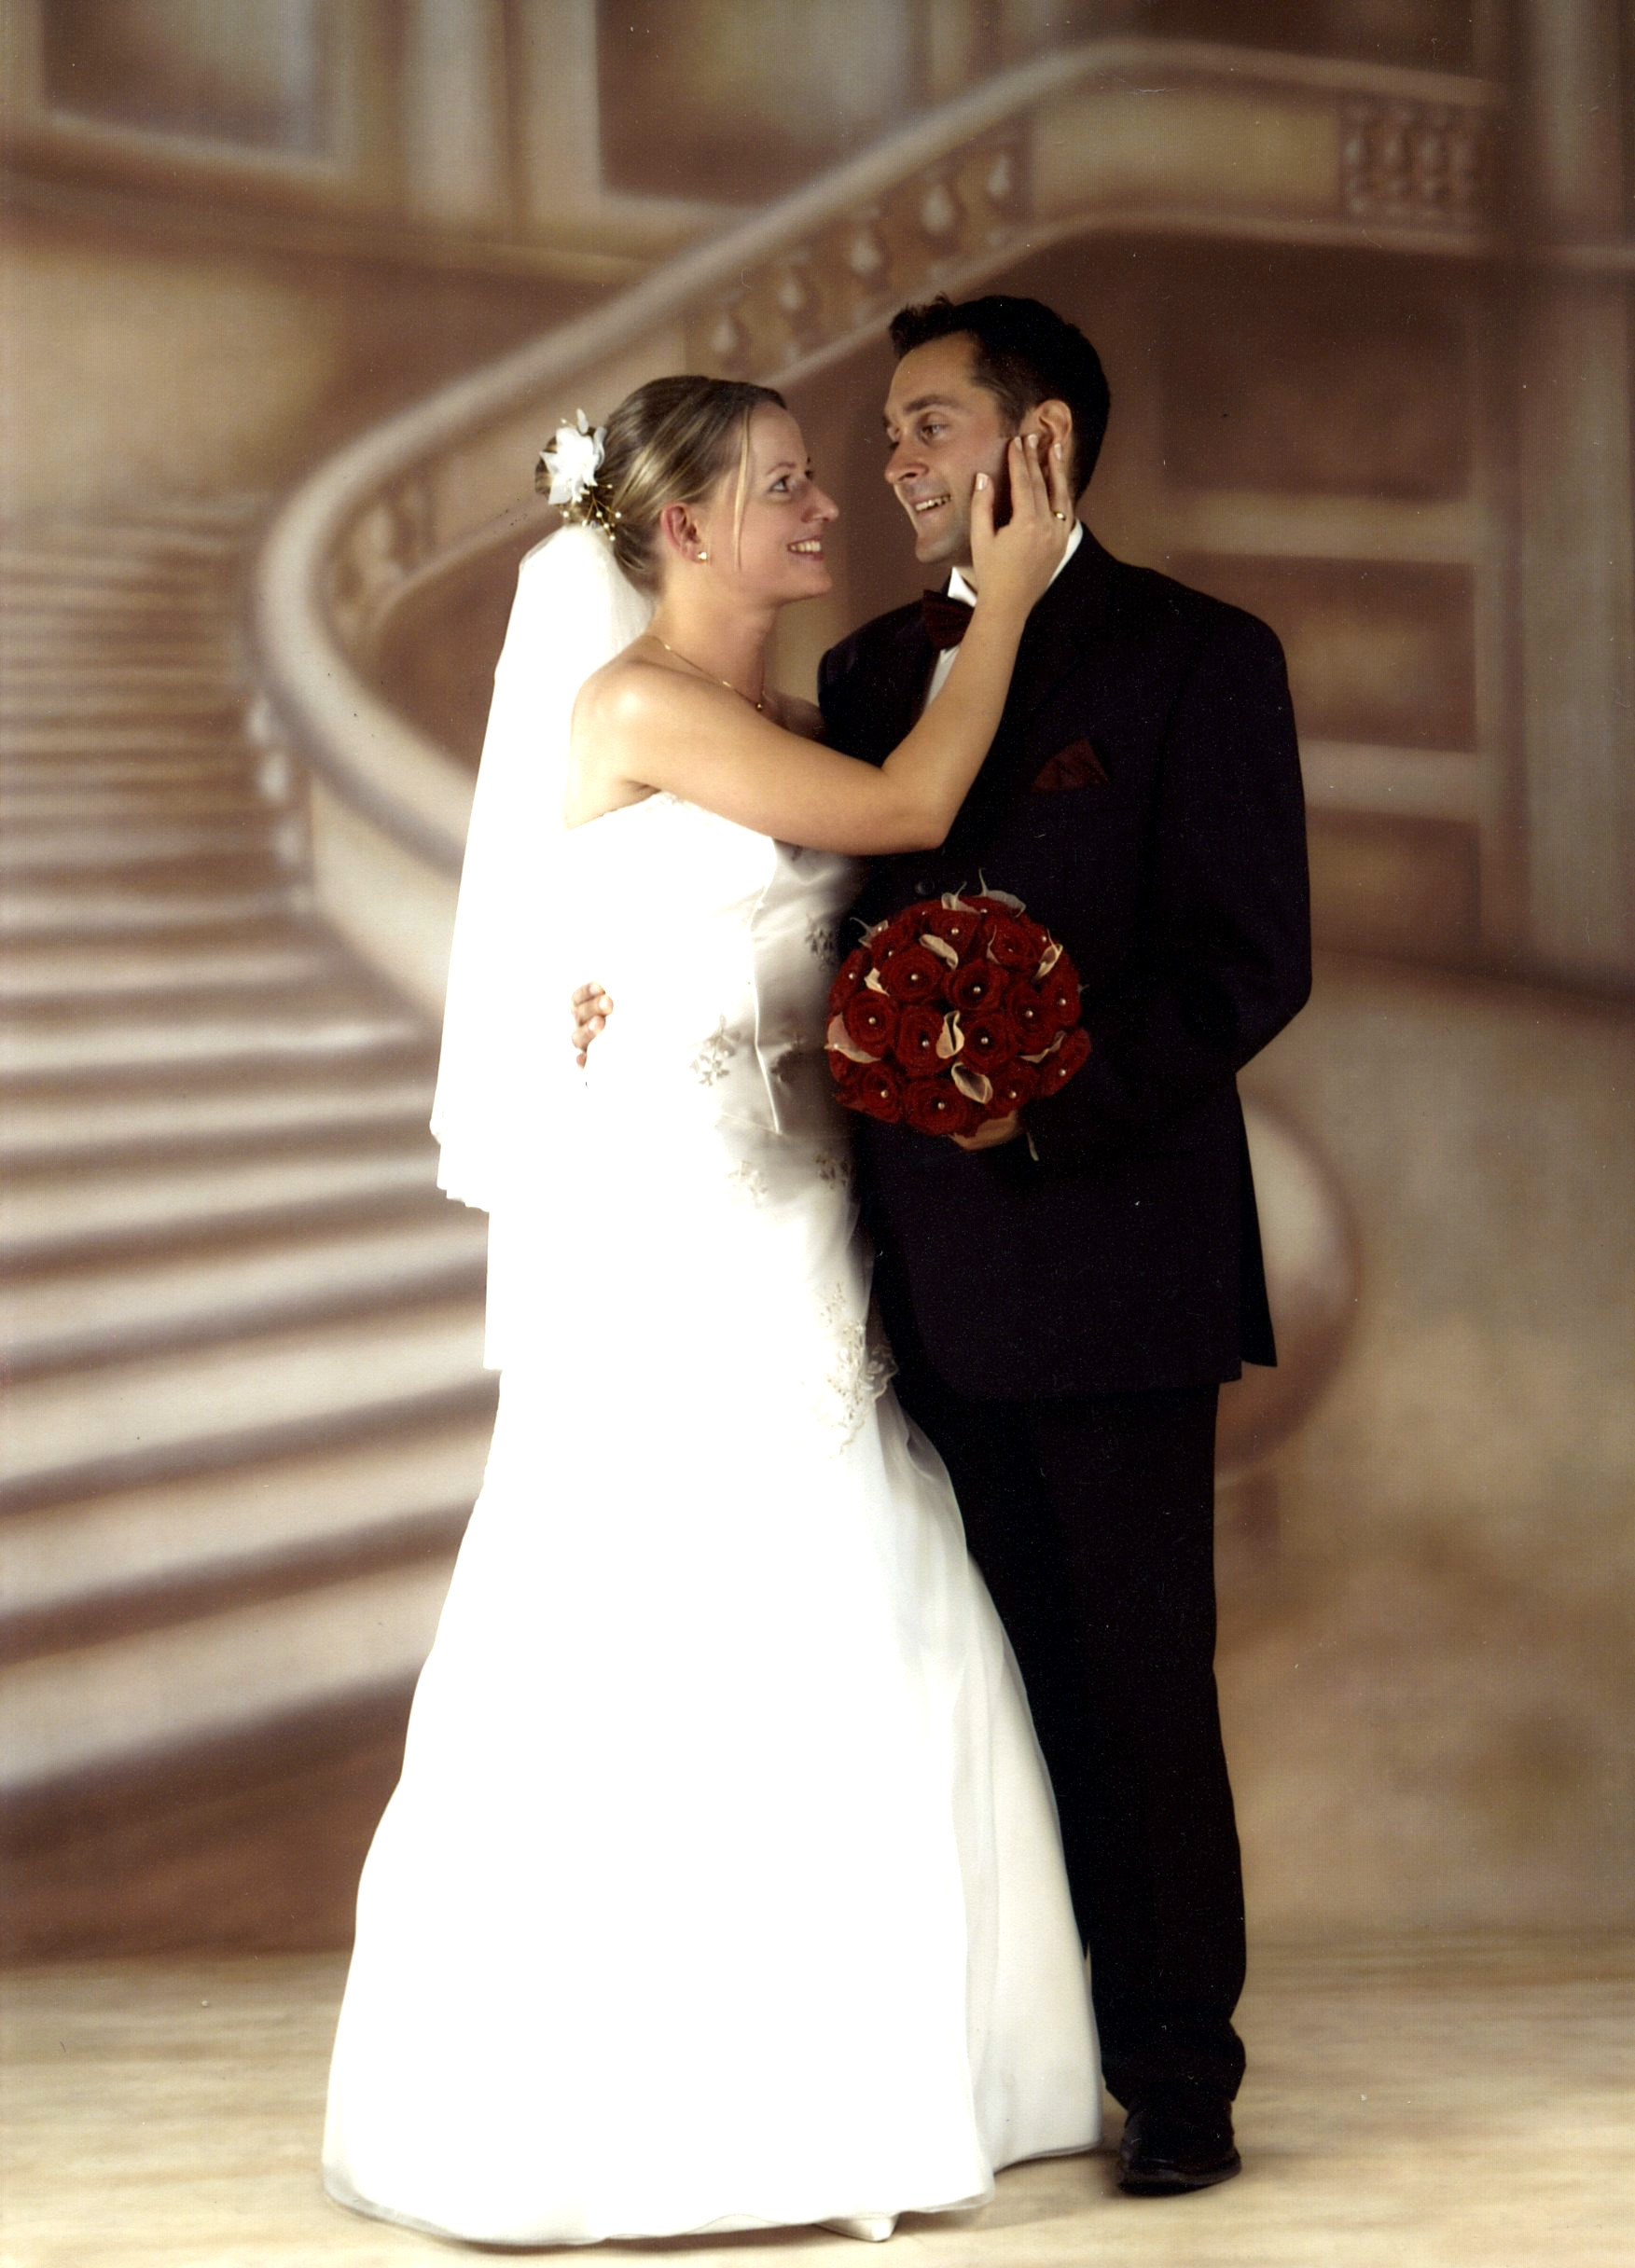
\includegraphics[width=0.3\textwidth]{photo/katarzyna_daniel_rybak_slub.jpg}
\caption{Ślub Katarzyny Kuś z Danielem Rybakiem}
\label{rys:katarzyna_daniel_rybak_slub}
\end{center}
\end{figure}

Mają \textbf{syna Cypriana ur. 18 listopada 2005~r. w Lublińcu}.

\textbf{Marcin ur. 6 marca 1979 r. w Lublińcu}, to najmłodszy syn Edwarda i Reginy.

Ukończył Wydział Mechaniki Samochodowej Politechniki Opolskiej z tytułem inżyniera, ale pracuje w firmie tapicerskiej w Lublińcu. Żona Marcina -- \textbf{Kinga Wojciechowska ur. 18~stycznia 1979~r. w Lublińcu z Jana i Eugenii z domu Krawczyk} ukończyła germanistykę w Częstochowie i uczy niemieckiego w lublinieckim ,,Medyku''.
\begin{figure}[!h]
\begin{center}
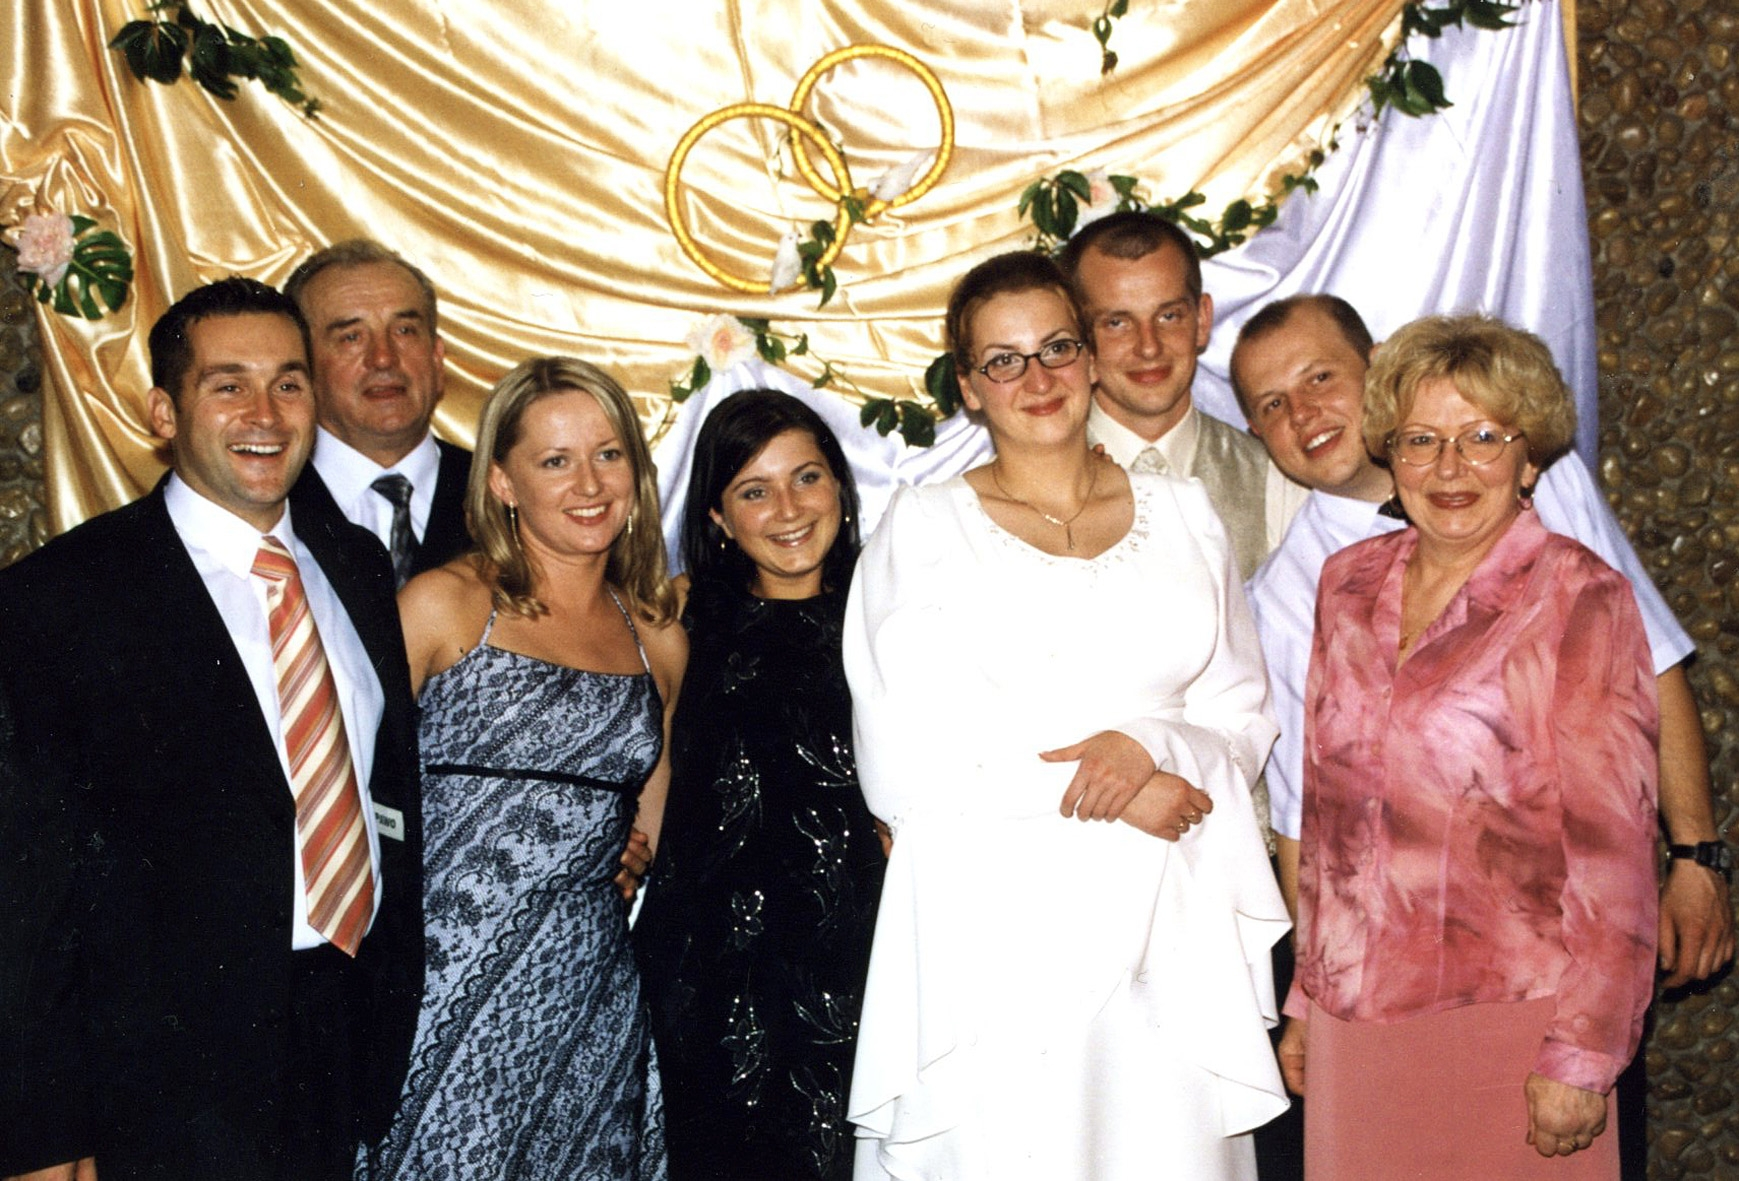
\includegraphics[height=40mm]{photo/marcin_kinga_kus_slub_2.jpg}
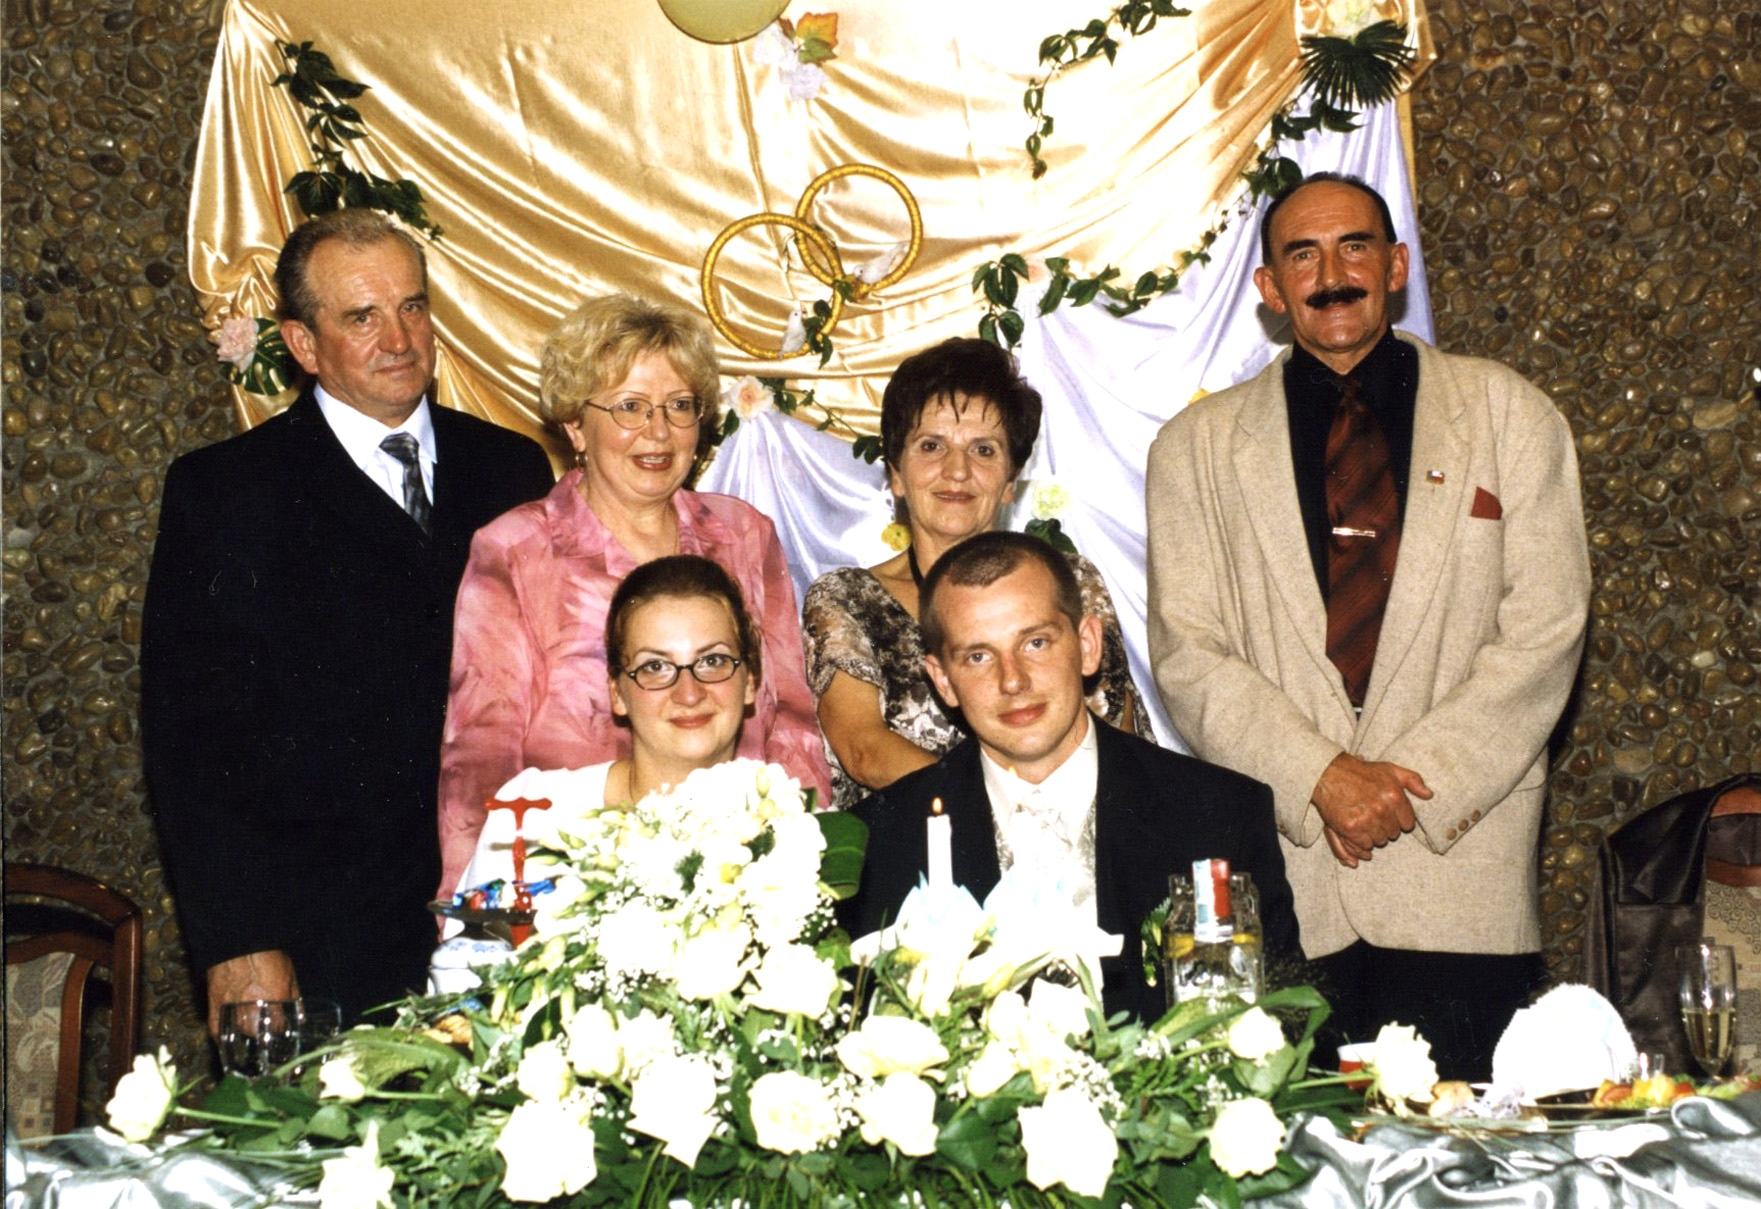
\includegraphics[height=40mm]{photo/marcin_kinga_kus_slub_3.jpg}
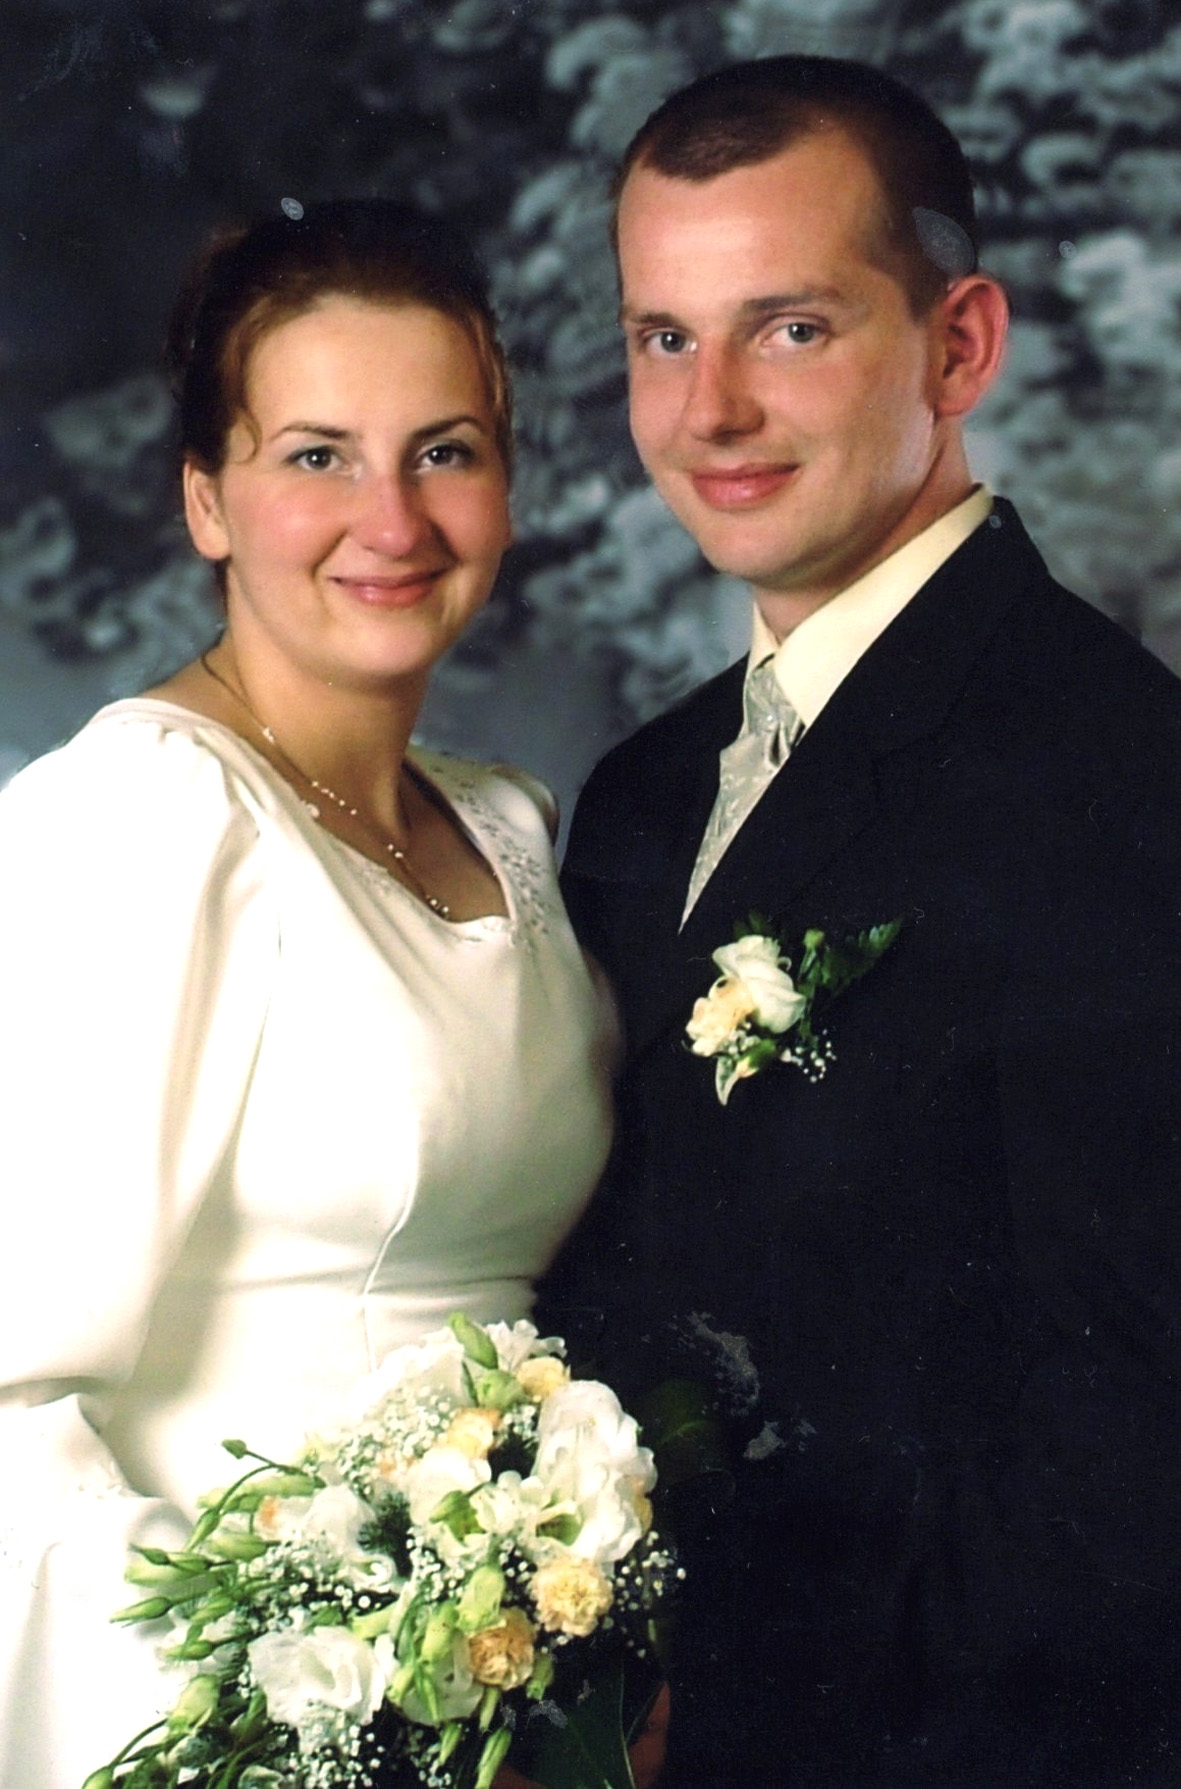
\includegraphics[height=40mm]{photo/marcin_kinga_kus_slub_1.jpg}
\caption[Zdjęcia ślubne Kingi Wojciechowskiej i Marcina Kusia]{Zdjęcia ślubne Kingi Wojciechowskiej i Marcina Kusia; na zdj. 11a od lewej: Daniel Rybak, Edward Kuś, Katarzyna Rybak, Agnieszka Kuś, Kinga Wojciechowska - Kuś, Marcin Kuś, Artur Kuś i Regina Kuś; na zdj. 11b za Kingą i Marcinem stoją ich rodzice: Edward i Regina Kusiowie oraz Eugenia i Jan Wojciechowscy; na zdj. 11c Kinga Wojciechowska z Marcinem Kusiem.}
\label{rys:marcin_kinga_kus_slub}
\end{center}
\end{figure}

\textbf{Mają syna Kamila ur. 5 marca 2005 r. w Lublińcu oraz córkę Dominikę Różę ur. 24 października 2008 r. w Lublińcu.}

Młodszy od Edwarda -- \textbf{Izydor Kuś przyszedł na świat 3 marca 1950~r}. Bardzo wiele nacierpiał się we wczesnym dzieciństwie najpierw w szpitalu w Chorzowie, a potem w domu, leżąc przez wiele miesięcy w ,,korytku gipsowym''.
\begin{figure} [!h]
\begin{center}
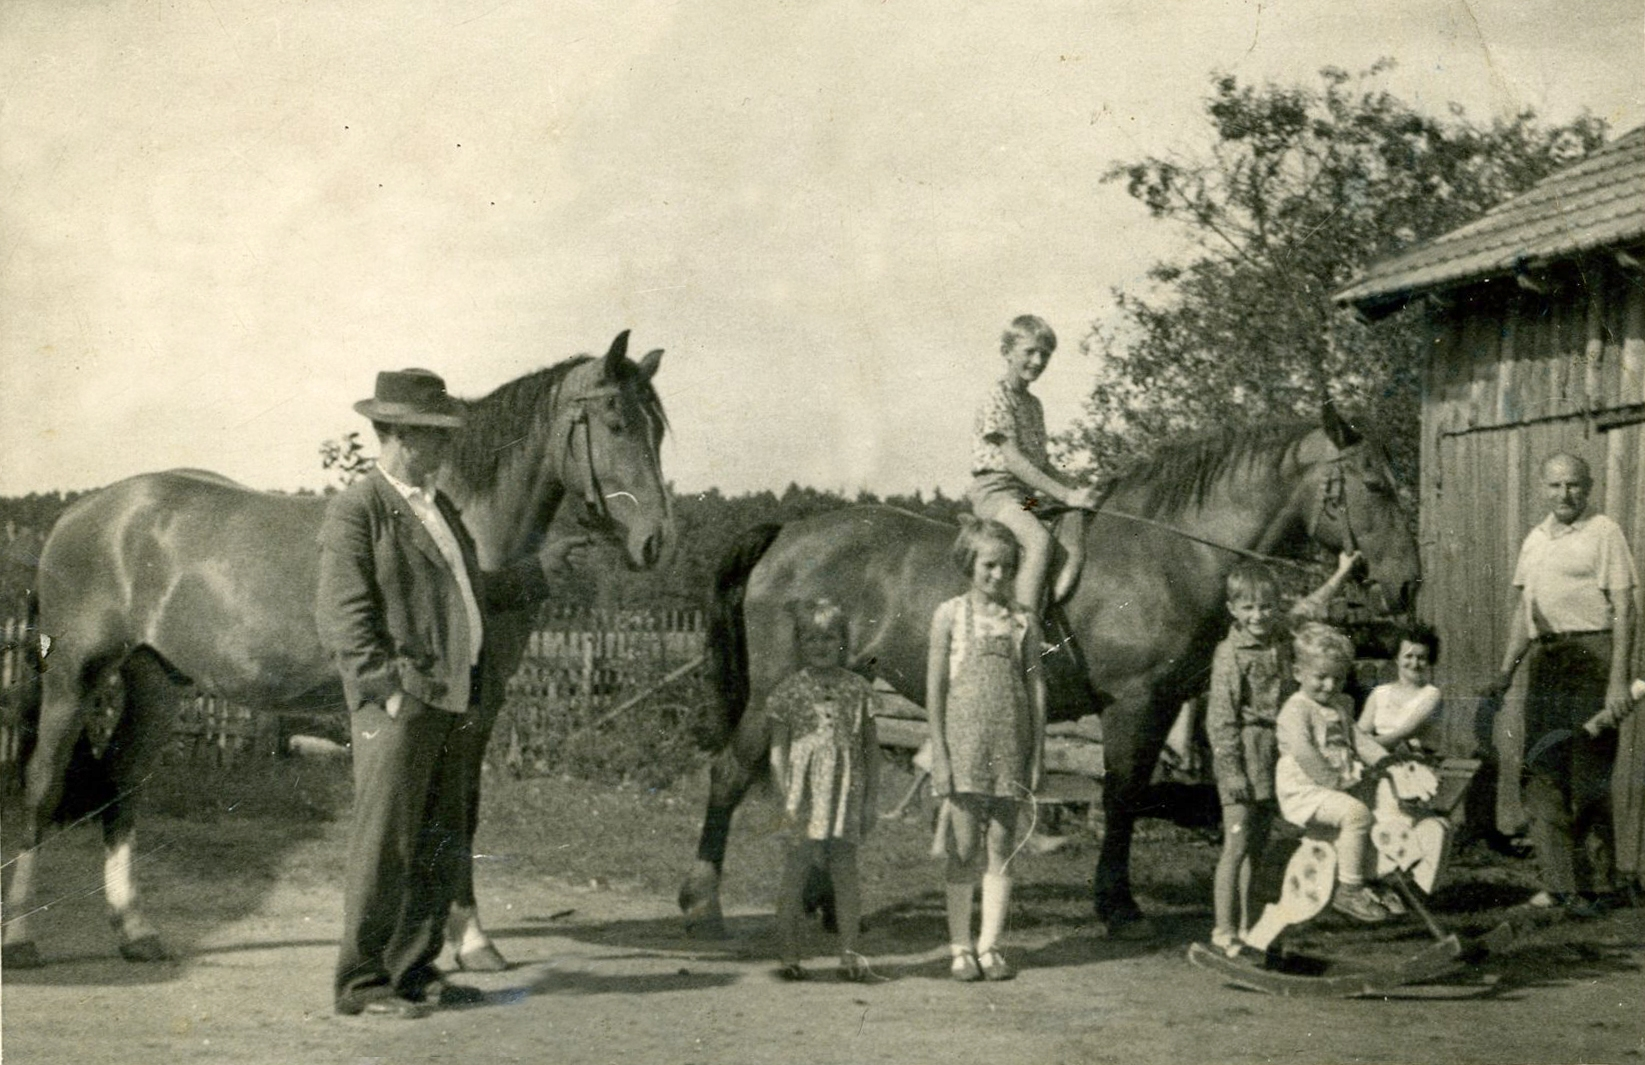
\includegraphics[width=0.7\textwidth]{photo/izydor_kus_1.jpg}
\caption[Kusiowie przy koniach]{Na zdj. Teodor Kuś trzyma konia za uzdę, na drugim koniu siedzi nasz Izydor Kuś, obok konia stoją Basia i Marysia Kusiówne, a Boguś Lehman trzyma tego konia za uzdę, przy nim na koniku bujanym siedzi Bogdan Kuś, obok siedzi babcia Radinka zaś przy szopie stoi stryj Antoni Lehman (mąż stryjenki Ireny).}
\label{rys:izydor_kus_1}
\end{center}
\end{figure}

Ukończywszy szkołę zawodową w zawodzie elektromonter, podjął pracę w Zakładzie Energetycznym w Lublińcu. Potem trzy lata pracował w POM-ie w Dobrodzieniu, a następnie w Rolniczej Spółdzielni Produkcyjnej w Pawonkowie, aż do jej rozwiązania, w związku z czym przeszedł na zasiłek przedemerytalny. Poza tym utrzymuje siebie i rodzinę z ćwiartki etatu w ogrodnictwie i jako operator koparko-ładowarki. \textbf{Ożenił się 13~kwietnia 1971~r. z Krystyną Jarzyną, córką Henryka z Tomaszowa Mazowieckiego i Gertrudy Polińskiej, urodzoną w Pawonkowie 15~lipca 1951~r.}
\begin{figure}[!h]
\begin{center}
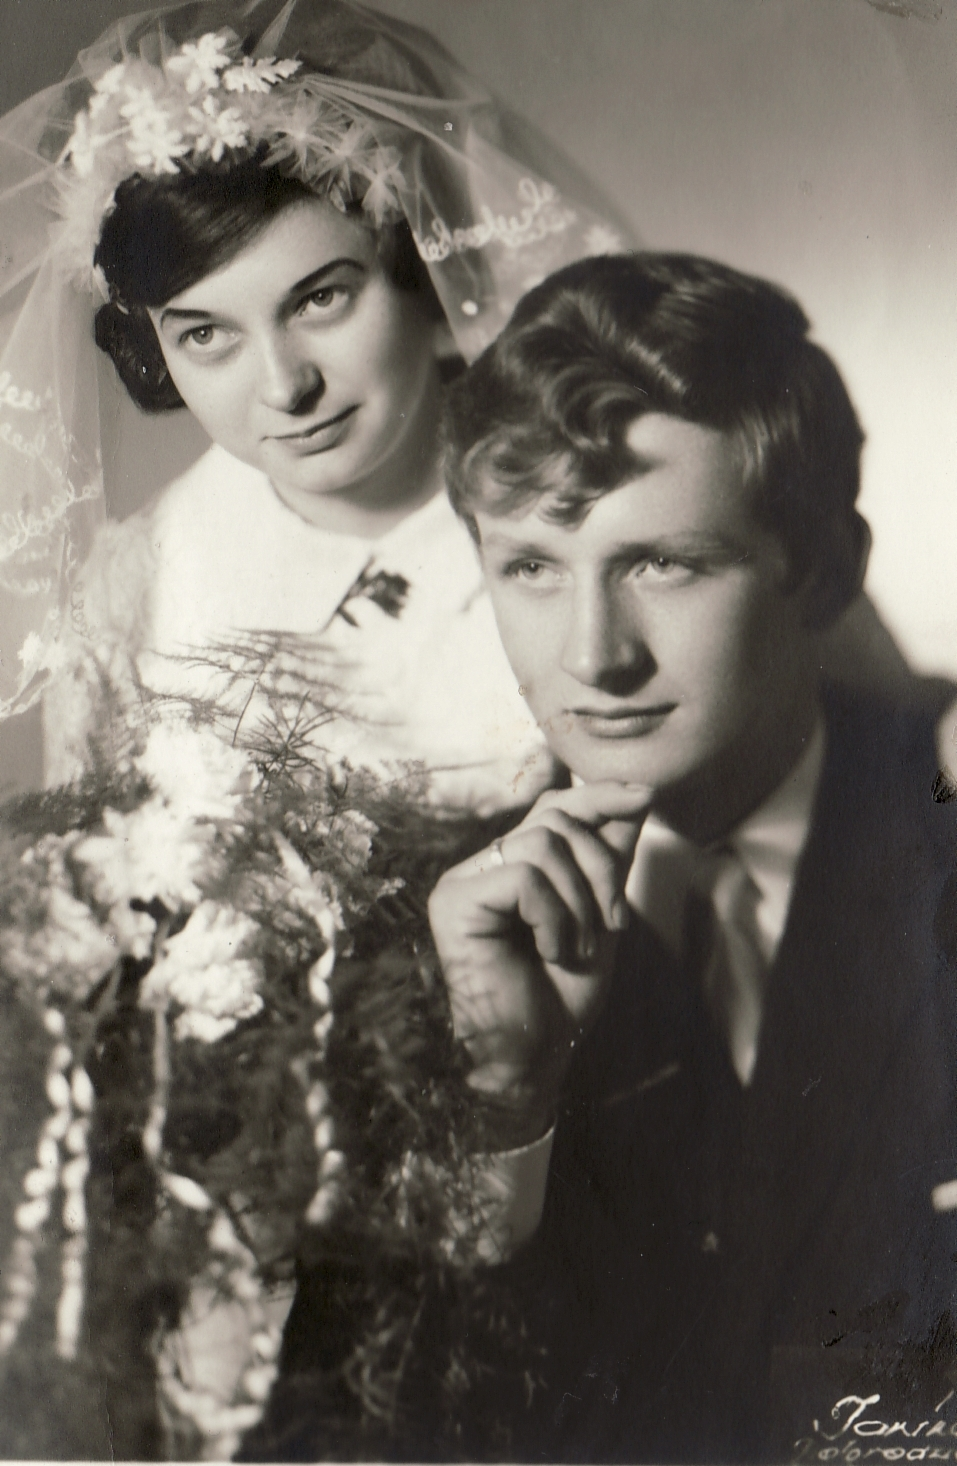
\includegraphics[height=60mm]{photo/izydor_krystyna_kus_slub_1.jpg}
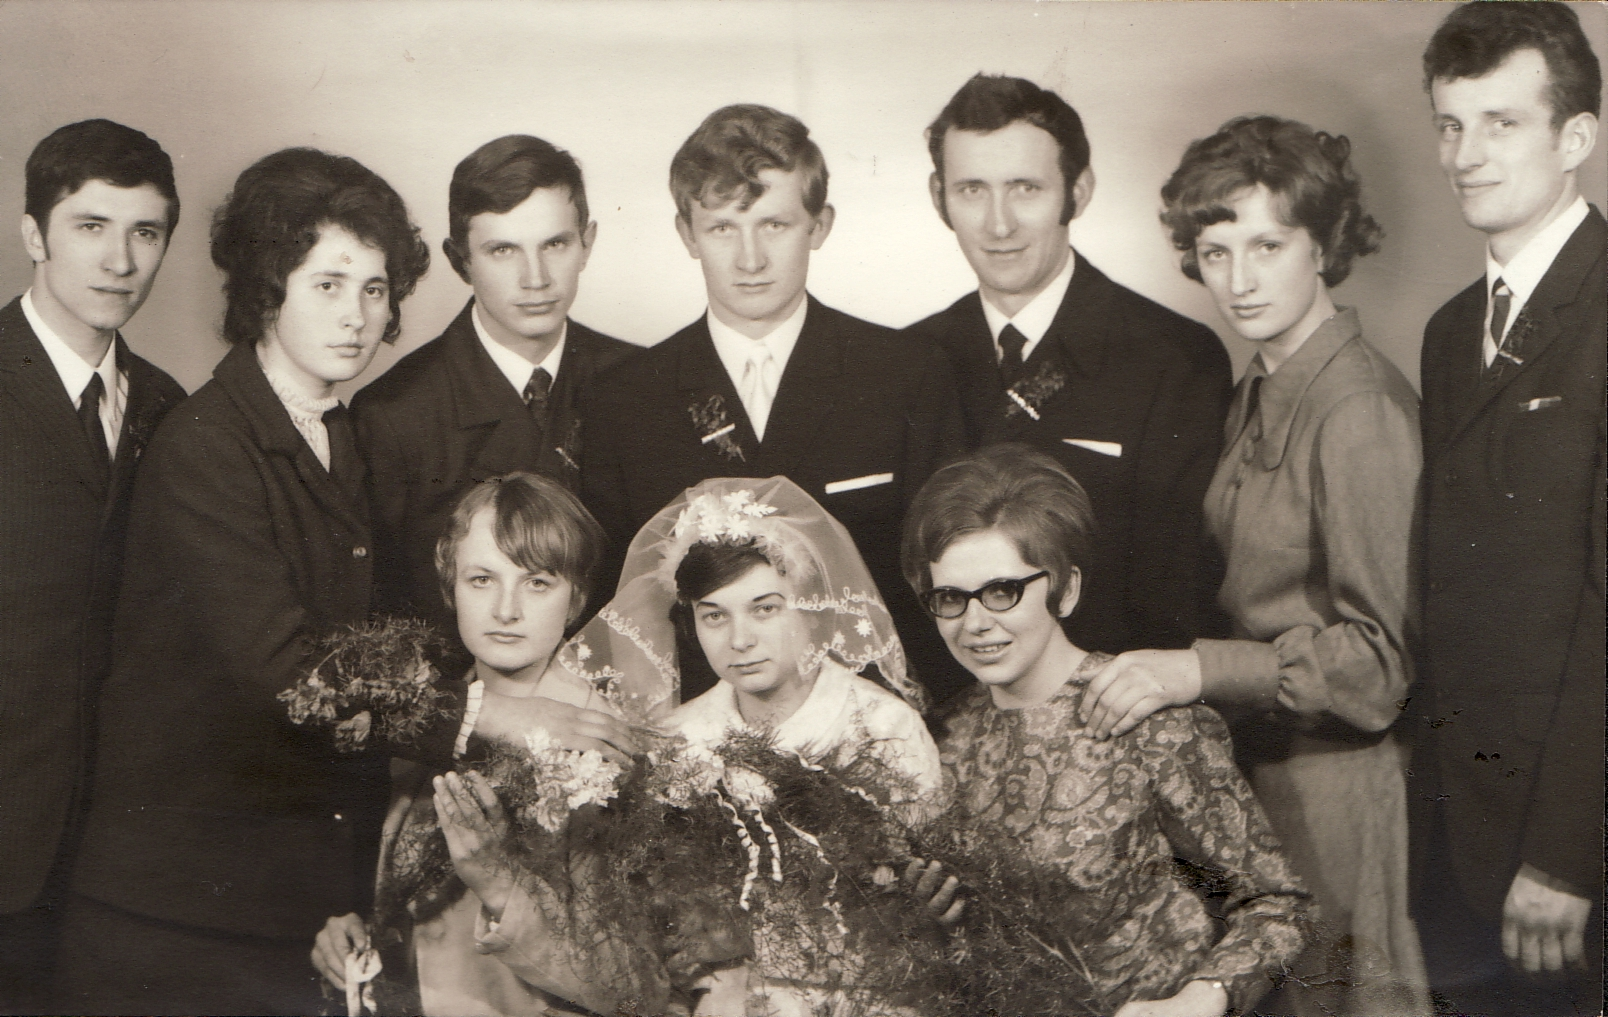
\includegraphics[height=60mm]{photo/izydor_krystyna_kus_slub_2.jpg}
\caption[Zdjęcia ślubne Krystyny Jarzyny i Izydora Kusia]{Zdjęcia ślubne Krystyny Jarzyny i Izydora Kusia. Na zdj. po prawej siedzą: Basia Kuś z Krystyną Jarzyną Kuś i Reginą Rurańską, za nimi stoją od lewej: NN i NN, Boguś Lehman,Izydor Kuś, Benedykt Klimza, Marysia Kuś i Edward Kuś.}
\label{rys:izydor_krystyna_kus_slub}
\end{center}
\end{figure}

\begin{figure}[!h]
\begin{center}
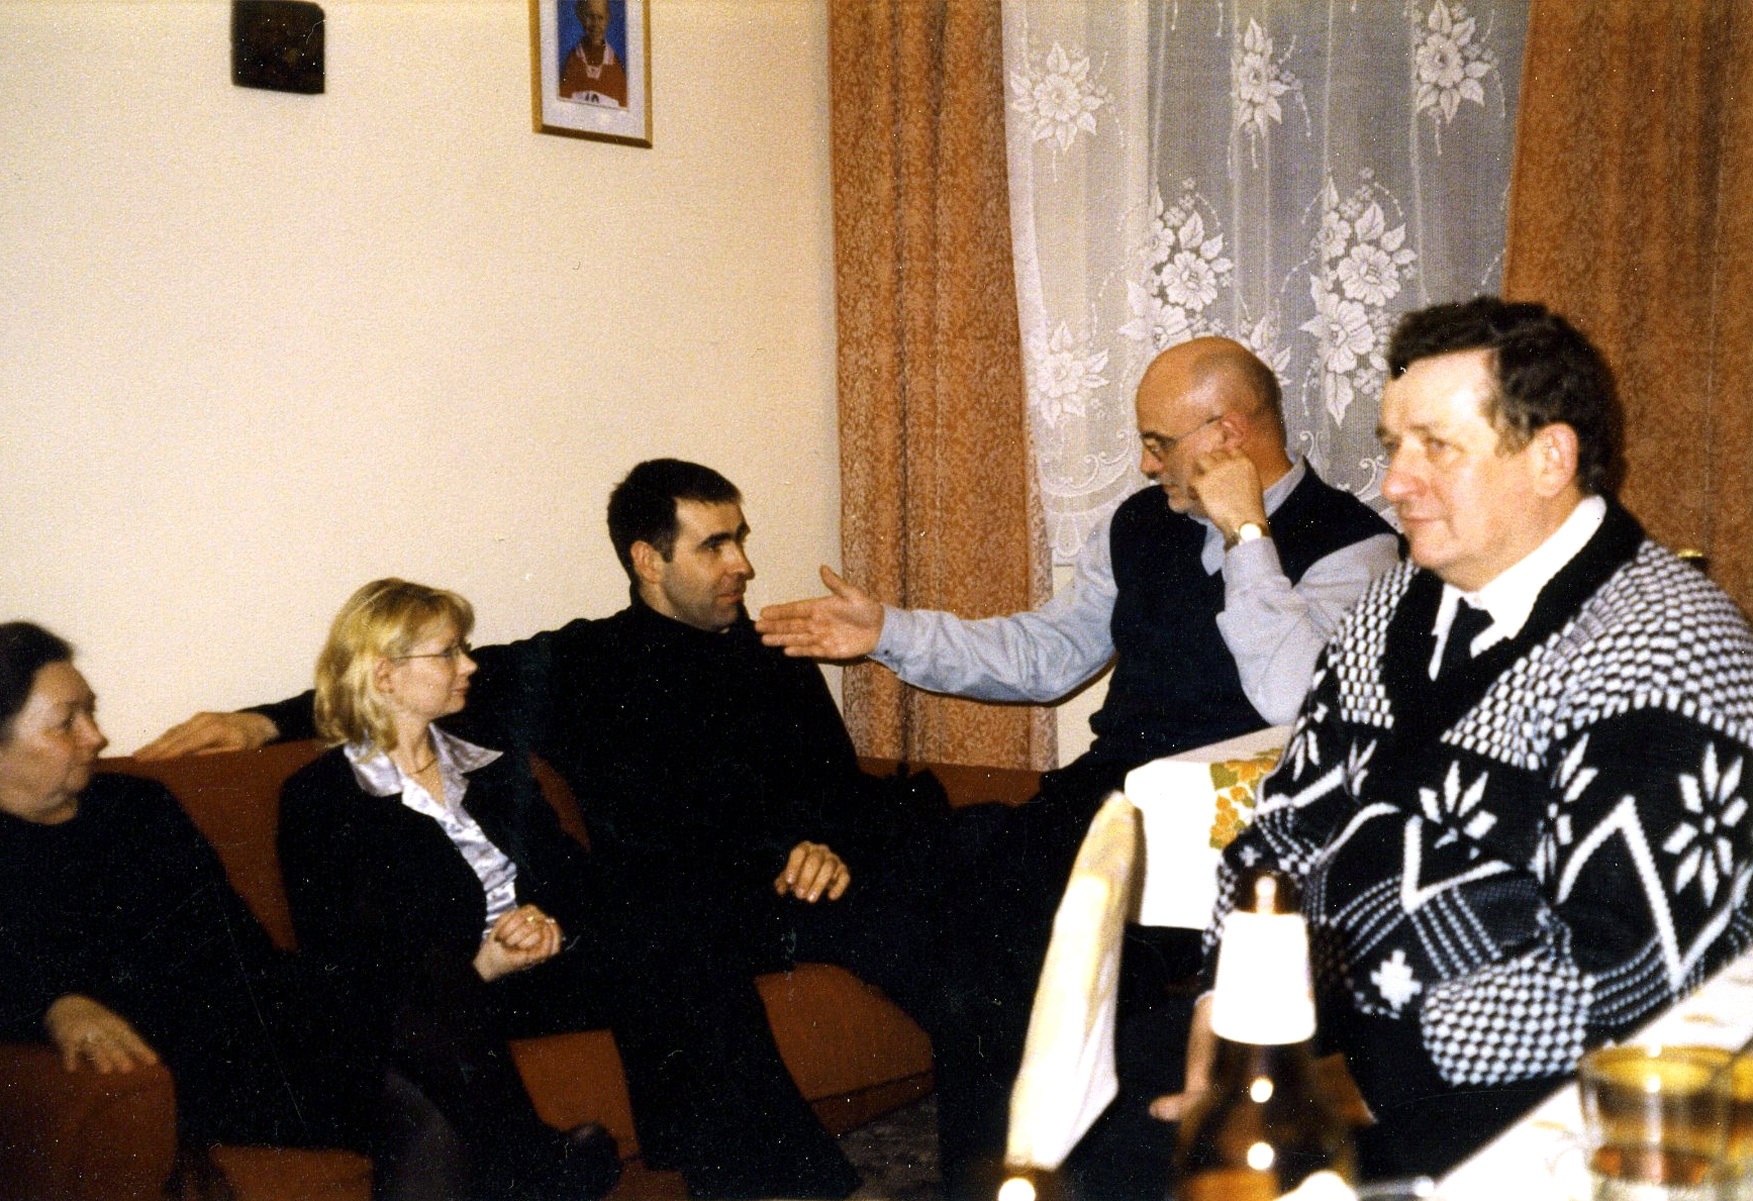
\includegraphics[width=0.6\textwidth]{photo/izydor_krystyna_kus_1.jpg}
\caption[Izydor Kuś]{Na zdj. od lewej: Krystyna Kuś, (żona Izydora) Danuta Kuś (ich córka), Andrzej Lehman (syn Tadeusza), Boguś Lehman oraz Izydor Kuś.}
\label{rys:izydor_krystyna_kus_1}
\end{center}
\end{figure}

Pracowała, po ukończeniu szkoły podstawowej, w Rolniczej Spółdzielni Produkcyjnej w Pawonkowie i stamtąd przeszła na rentę chorobową. \textbf{Mają córkę Danutę urodzoną 19~czerwca 1971~r. w Lublińcu}, która ukończywszy Technikum Odzieżowe w Tarnowskich Górach, zatrudniła się w firmie ,,Meble~-~Kler'' w Dobrodzieniu.

Mieszka z rodzicami w domu, który wybudował sobie Izydor na wykupionej przez siebie działce w Pawonkowie przy ul. Kwiatowej 12. Mieszka z nimi jego teściowa -- Gertruda.

\textbf{Marysia Kusiówna} -- najstarsza córka Róży i Teodora -- \textbf{przyszła na świat 8 grudnia 1952 r. w Łagiewnikach Wielkich}.
\begin{figure}[!h]
\begin{center}
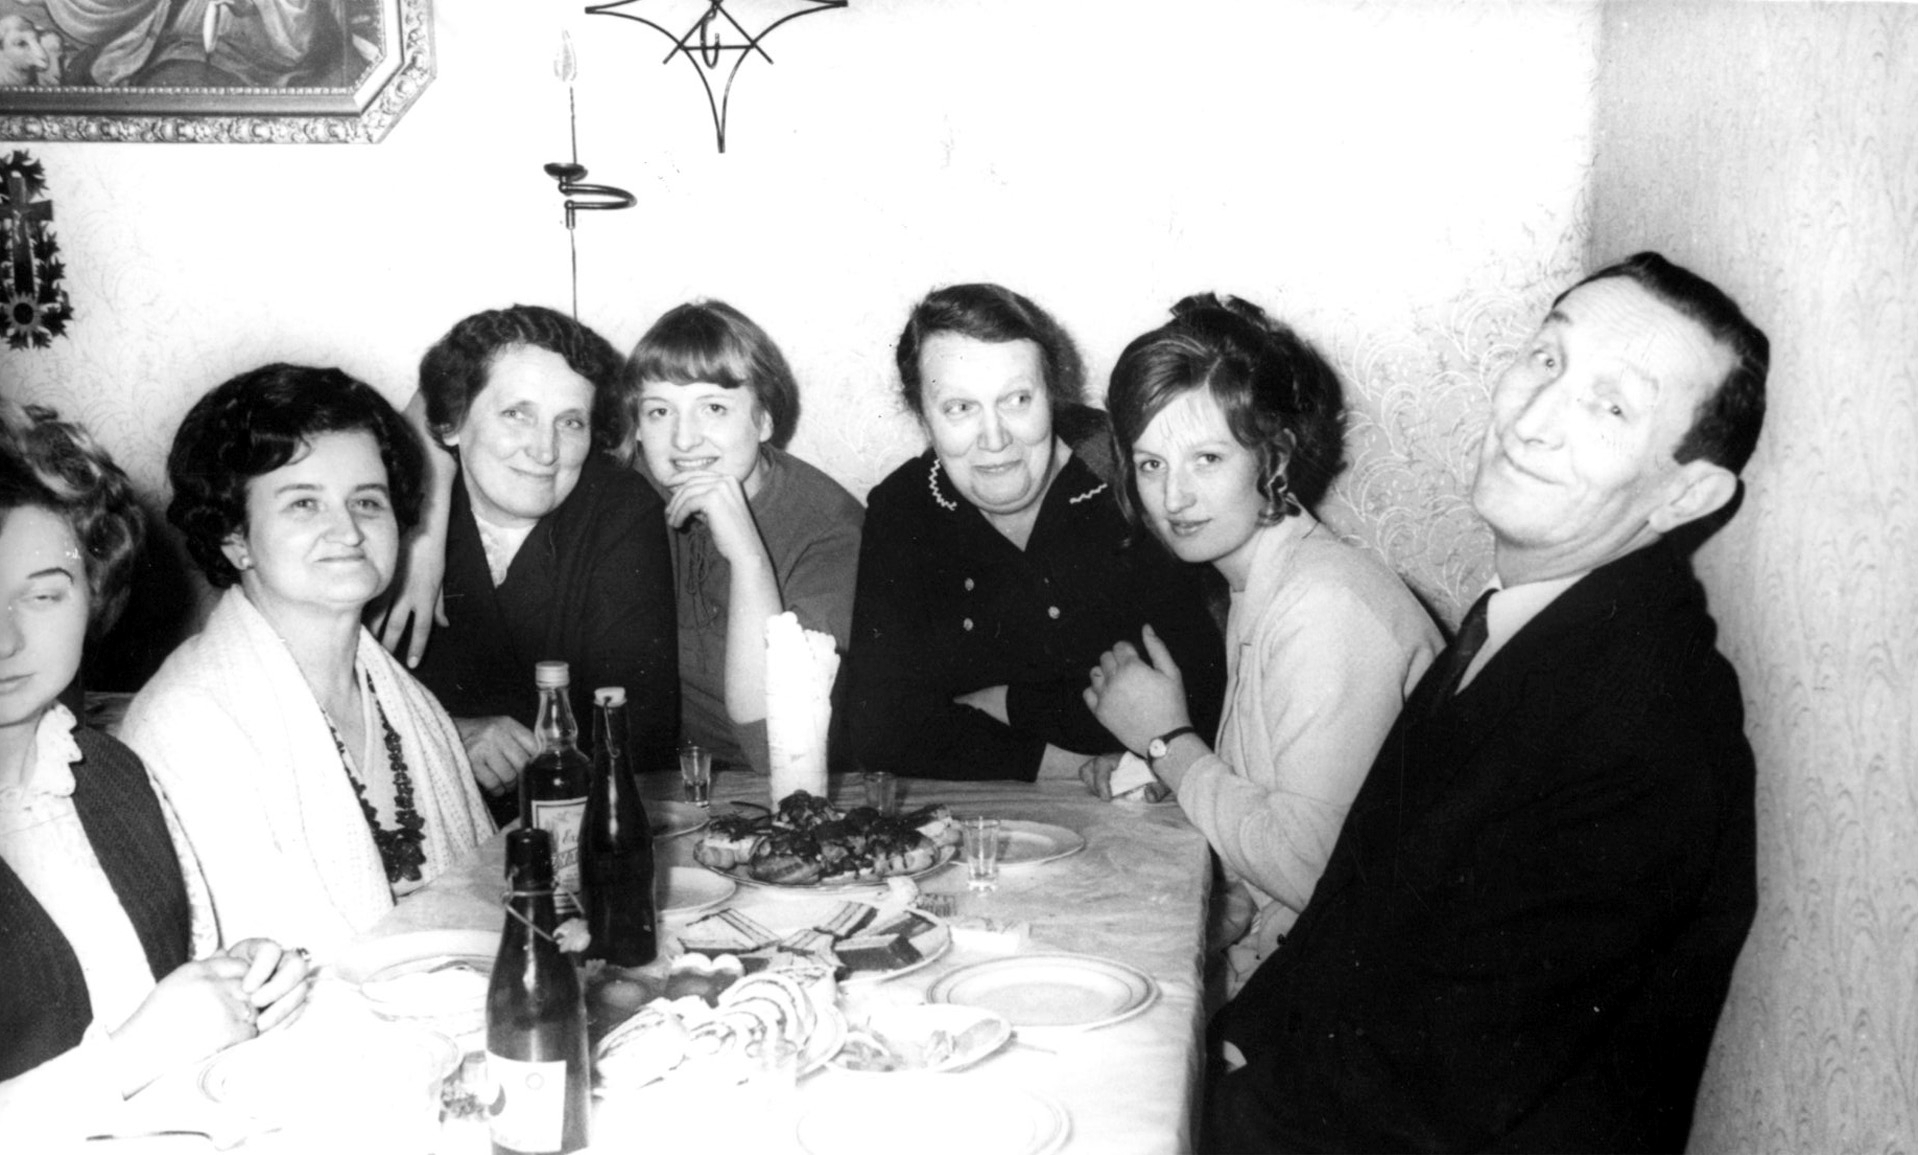
\includegraphics[width=0.6\textwidth]{photo/maria_kus_1.jpg}
\caption[Marysia Kuś]{Na zdj. od lewej: babcia Radinka Świerczyńska, Rózia Kuś, Basia Kuś (córka Rózi), Irena Lehman, Marysia Kuś i dziadek Benedykt Świerczyński.}
\label{rys:maria_kus_1}
\end{center}
\end{figure}

\begin{figure}[!h]
\begin{center}
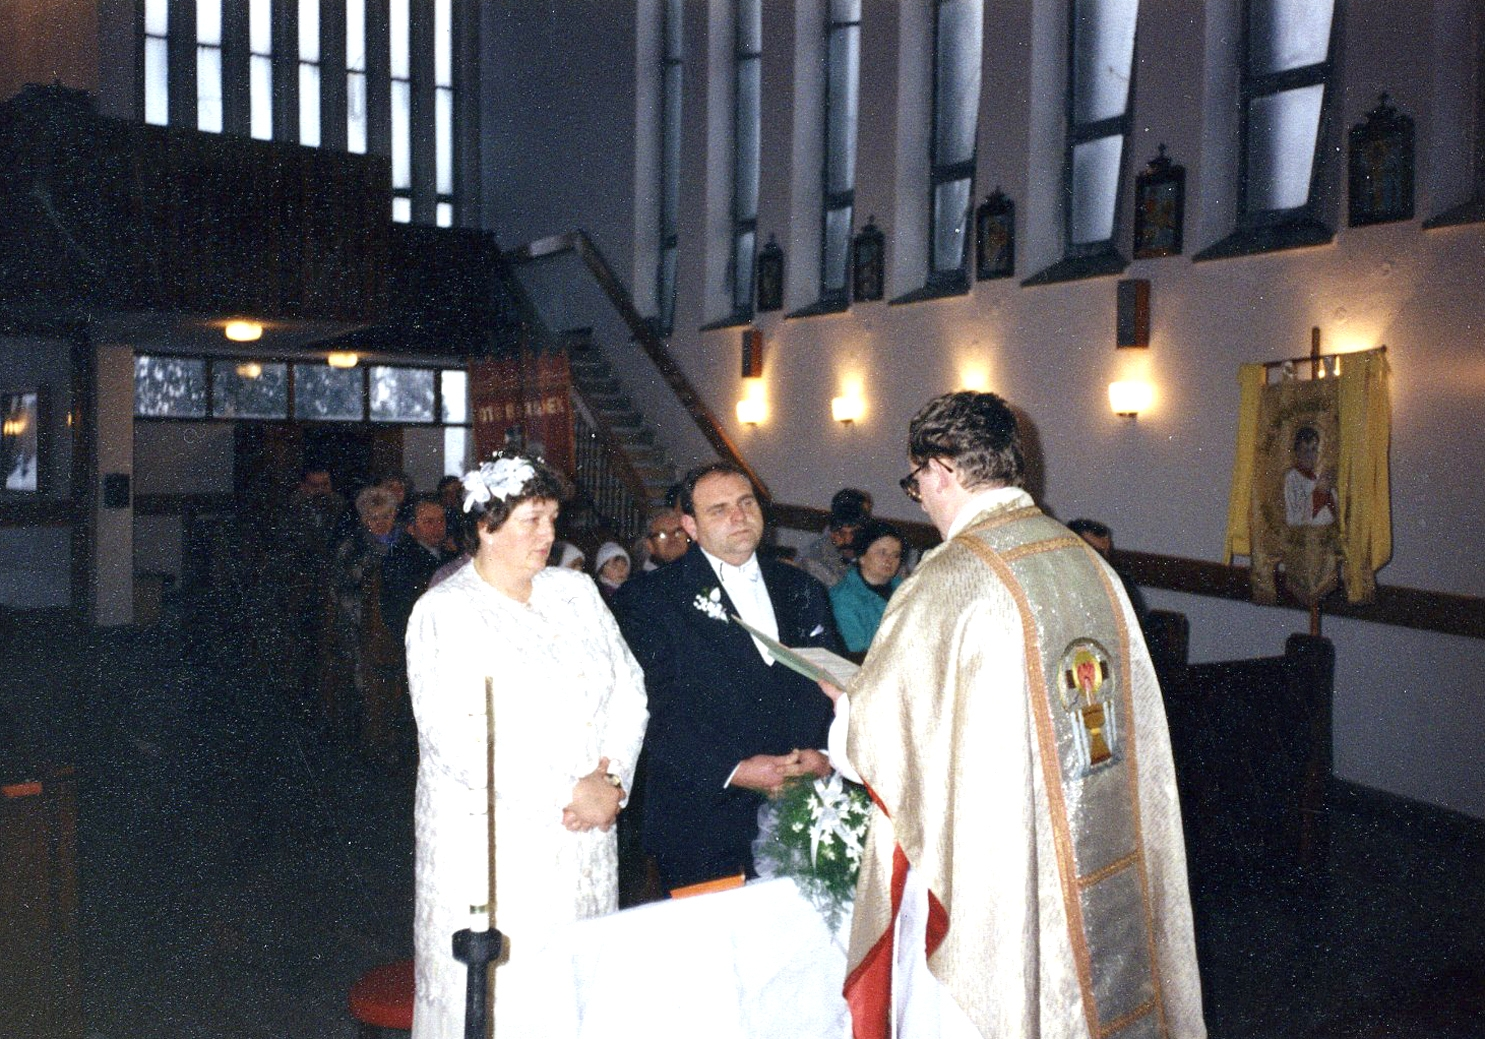
\includegraphics[width=0.6\textwidth]{photo/maria_bernard_sprycha_slub.jpg}
\caption{Zdjęcie ślubne Marysi Kuś i Bernarda Sprychy}
\label{rys:maria_bernard_sprycha_slub}
\end{center}
\end{figure}

Po latach ukończyła Liceum Ogólnokształcące dla Pracujących w Lublińcu. Utrzymywała się z pracy w PZGS od 1972~r. W 1990 r. podjęła pracę w Ośrodku Szkolno Wychowawczym dla Niesłyszących lub Słabosłyszących w Lublińcu jako magazynierka i pracuje tam do dziś. Poznała tam stolarza po Zawodowej Szkole Stolarskiej w Dobrodzieniu - \textbf{Bernarda Sprychę ur. 30 lipca 1958~r. w Lublińcu z Pawła i Marii z domu Fyrlus}.

\textbf{Pobrali się 29 grudnia 1992 r. w Łagiewnikach Wielkich.}

Zanim Bernard przeszedł na rentę chorobową, wybudowali sobie dom w Glinicy przy ul. Białej 16. \textbf{Nie mają dzieci}.

\begin{figure}[!h]
\begin{center}
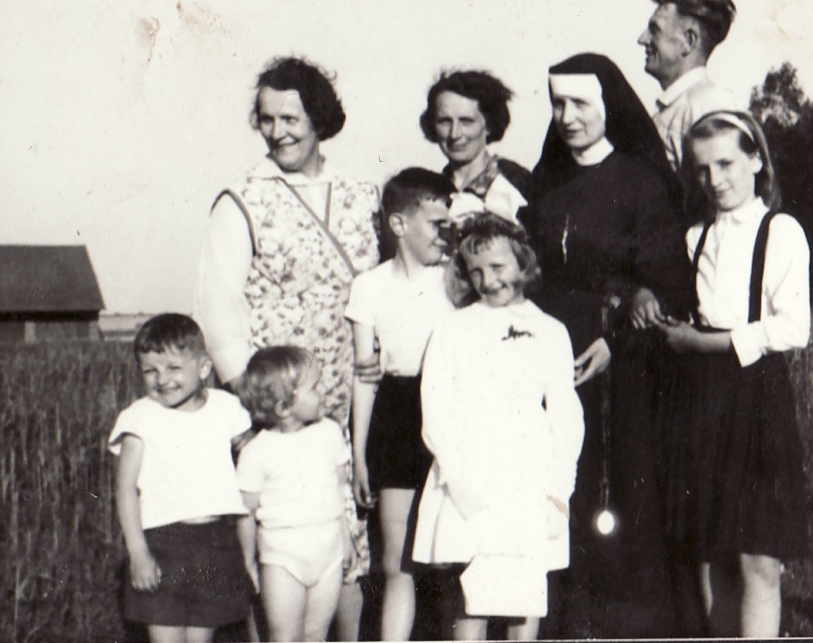
\includegraphics[width=0.55\textwidth]{photo/barbara_kus_komunia.jpg}
\caption[Pierwsza Komunia św. Barbary Kuś]{Pierwsza Komunia św. Barbary Kuś, na zdj. od lewej: Bogdan Kuś, Grzesiu Lehman - wnuk stojącej za nim Ireny Lehman, Boguś Lehman - jej syn, Basia z Marysią Kuś, za nimi od lewej Irena Lehman, Rózia Kuś, s. Aurelia Świerczyńska i za nią Teodor Kuś.}
\label{rys:barbara_kus_komunia}
\end{center}
\end{figure}

W trzy lata po Marysi -- \textbf{4 grudnia 1955 r. w Lublińcu przyszła na świat Barbara Kusiówna}, która po ukończeniu Liceum Medycznego w Mikołowie podjęła pracę w Szpitalu Zakaźnym w Lublińcu, a następnie w Szpitalu w Zawadzkiem. Po jego likwidacji kontynuuje pracę pielęgniarki w ZOZ-ie w Strzelcach Opolskich, dokąd dojeżdża korzystając z uprzejmości dobrych ludzi i \textbf{męża -- Zdzisława Walotka ur. 22 listopada 1954 r. w Lublińcu, syna Mieczysława Walotka z Chruszczobrodu} (jego dziadek natomiast pisał się Walutek) \textbf{oraz Teresy Suchary}.

\begin{figure}[!h]
\begin{center}
\includegraphics[height=50mm]{photo/barbara_zdzislaw_walotkowie_slub_1.jpg}
\includegraphics[height=50mm]{photo/barbara_zdzislaw_walotkowie_slub_2.jpg}
\caption{Ślub Barbary Kuś i Zdzisława Walotka}
\label{rys:barbara_zdzislaw_walotkowie_slub}
\end{center}
\end{figure}

Po ukończeniu Szkoły Zawodowej w zawodzie Elektromonter pracował w Hucie ,,Zawadzkie'' do jej likwidacji w 2004 r. jako kierowca zakładowej straży pożarnej, skąd odszedł na emeryturę i do 2007 r. dorabiał sobie w firmie ochroniarskiej ,,alfa''. \textbf{Pobrali się 1 października 1977r. w~Łagiewnikach Wielkich.}

Mieszkają w bloku w Zawadzkiem przy ul. Opolskiej 61. W Lublińcu mają dom jednorodzinny przy ul. Oleskiej 15a, gdzie mieszka mama Zdzisława Walotka. \textbf{Mają dwie córki: Aleksandrę i Agatę.}

\textbf{Aleksandra urodzona 18 listopada 1978 r. w Lublińcu} ukończyła pomaturalną Ochronę Praw, a później uzyskała licencjat po studiach z resocjalizacji w Opolu. Wyjechała szukać szczęścia w Niemczech. Mieszka w Mannheim, gdzie ukończyła szkołę Pomocy Pielęgniarskiej i szuka pracy. \textbf{Wyszła za Torstena Weimanna ur. 1 czerwca 1981~r. w Mannheim z Klausa i Ellen z domu Walter.}

\textbf{Dnia 2 grudnia 2008 r. urodziła syna Juliana.}

\textbf{Agata, jej siostra, urodzona 12 lipca 1995 r. w Lublińcu} ukończyła tam Liceum Ogólnokształcące i po maturze pojechała do siostry do Niemiec i tam mieszka.


Dziedzicem majątku Róży Świerczyńskiej Kuś i Teodora Kusia jest ich najmłodszy syn -- \textbf{Bogdan Kuś urodzony 19 sierpnia 1959~r. w~Łagiewnikach Wielkich}.

W 1976 r. ukończył Zasadniczą Szkołę Rolniczą w Lublińcu, gdzie poznał swoją przyszłą małżonkę -- pannę \textbf{Marysię Pytel z Harbułtowic}.

\begin{figure}[!h]
\begin{center}
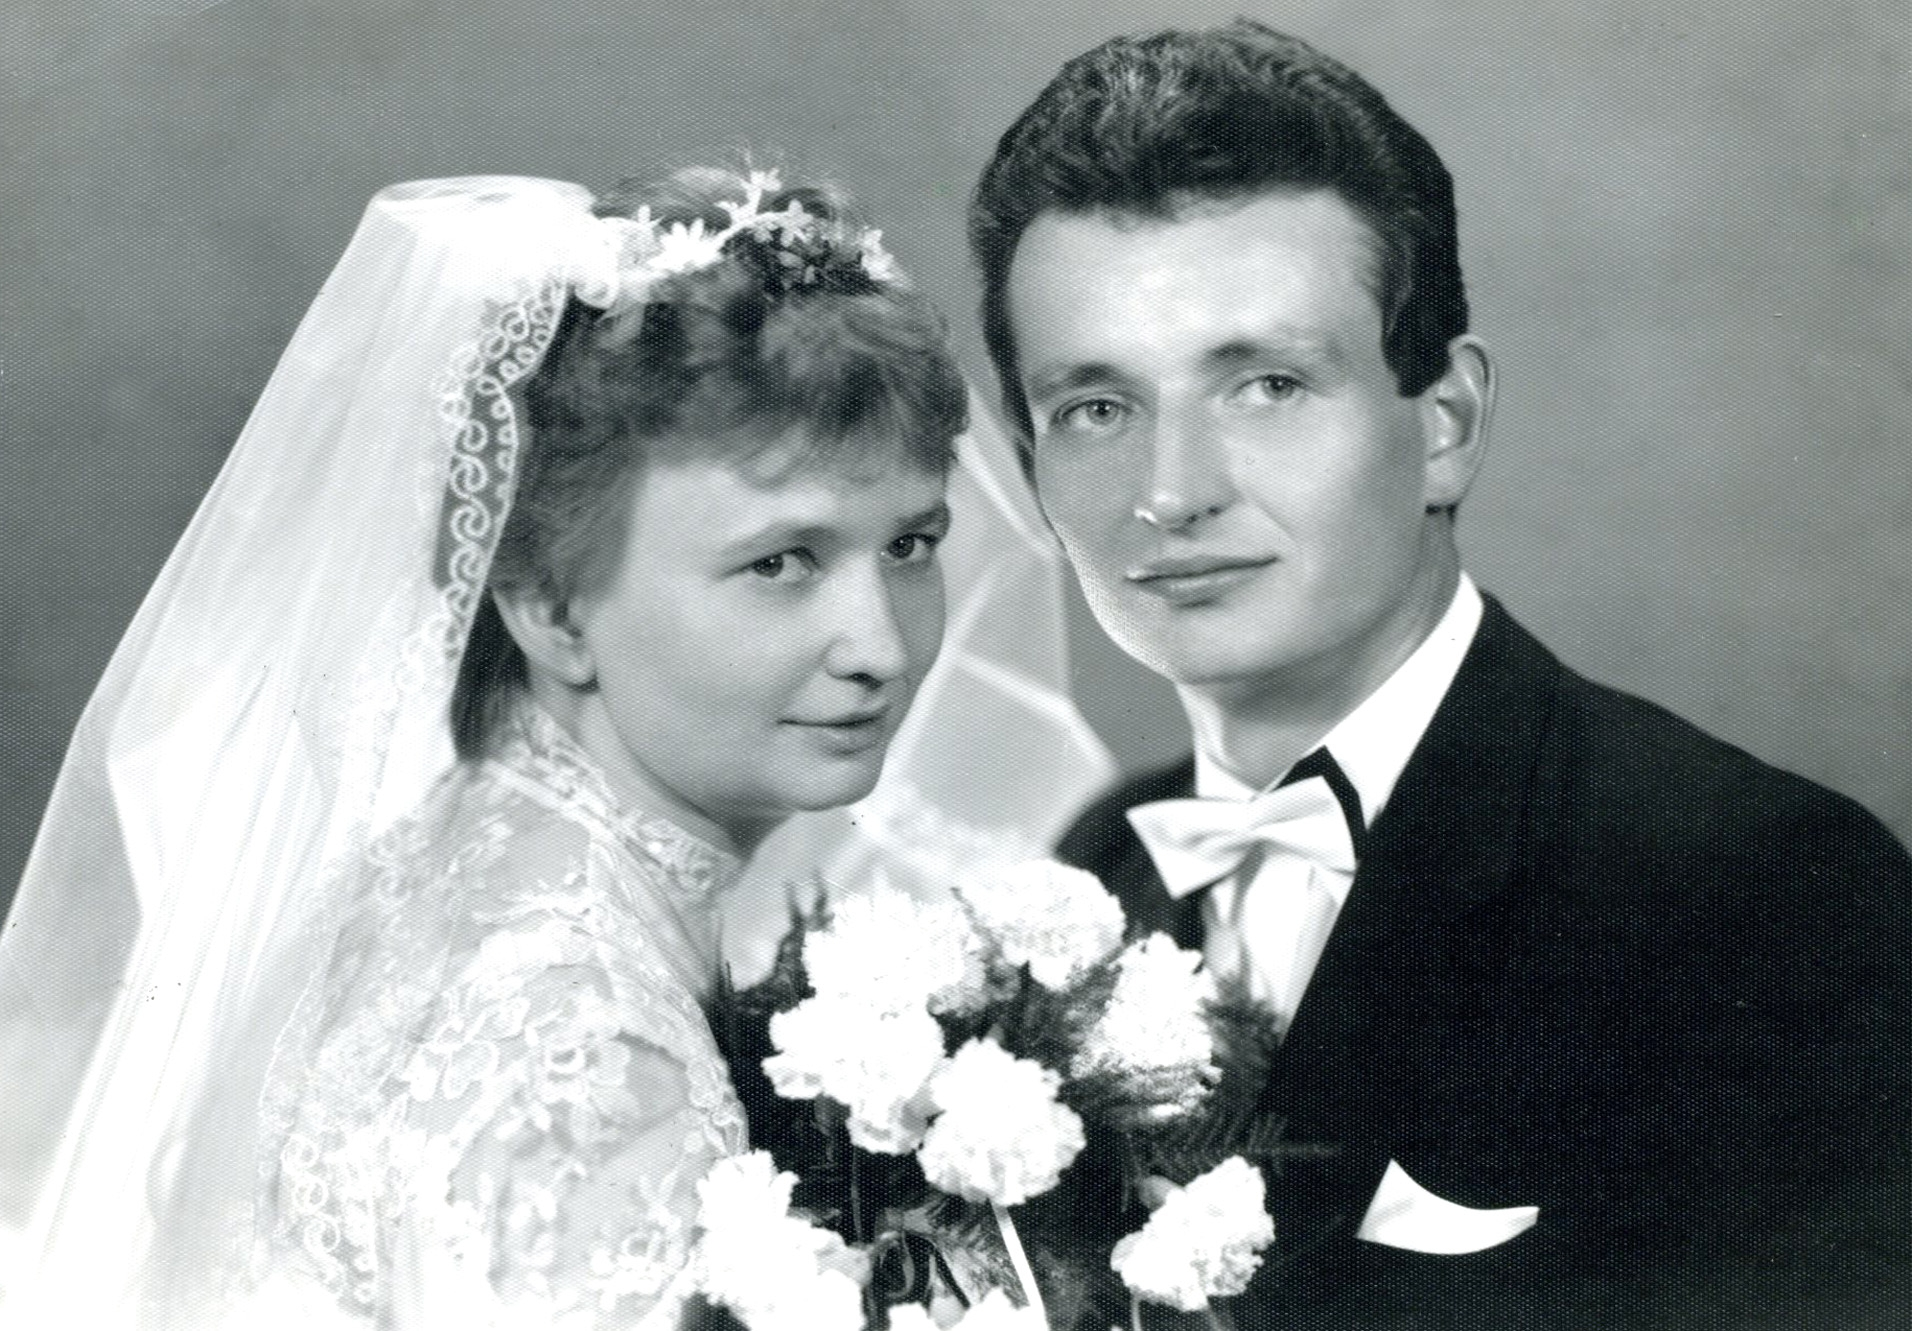
\includegraphics[width=0.55\textwidth]{photo/bogdan_marysia_kus_slub_1.jpg}
\caption{Ślub Marysi Pytel i Bogdana Kusia}
\label{rys:bogdan_marysia_kus_slub_1}
\end{center}
\end{figure}

\textbf{Urodziła się ona 13 października 1959 r. w Koszęcinie z ojca Franciszka Pytla (ur. 5 VII 1917~r. – zm. 20 XI 1966~r.) i matki Emilii z domu Toma (ur. 15 IX 1919~r. – zm. 15 VI 2001~r.).}

Kontynuowała naukę w Technikum Rolniczym w Złotym Potoku, które ukończyła w 1979r. \textbf{Pobrali się 20 września 1986 r. w Sadowiu i mają jednego syna – Adama ur. 12 lipca 1995 r. w Lublińcu.}

\begin{figure}[!h]
\begin{center}
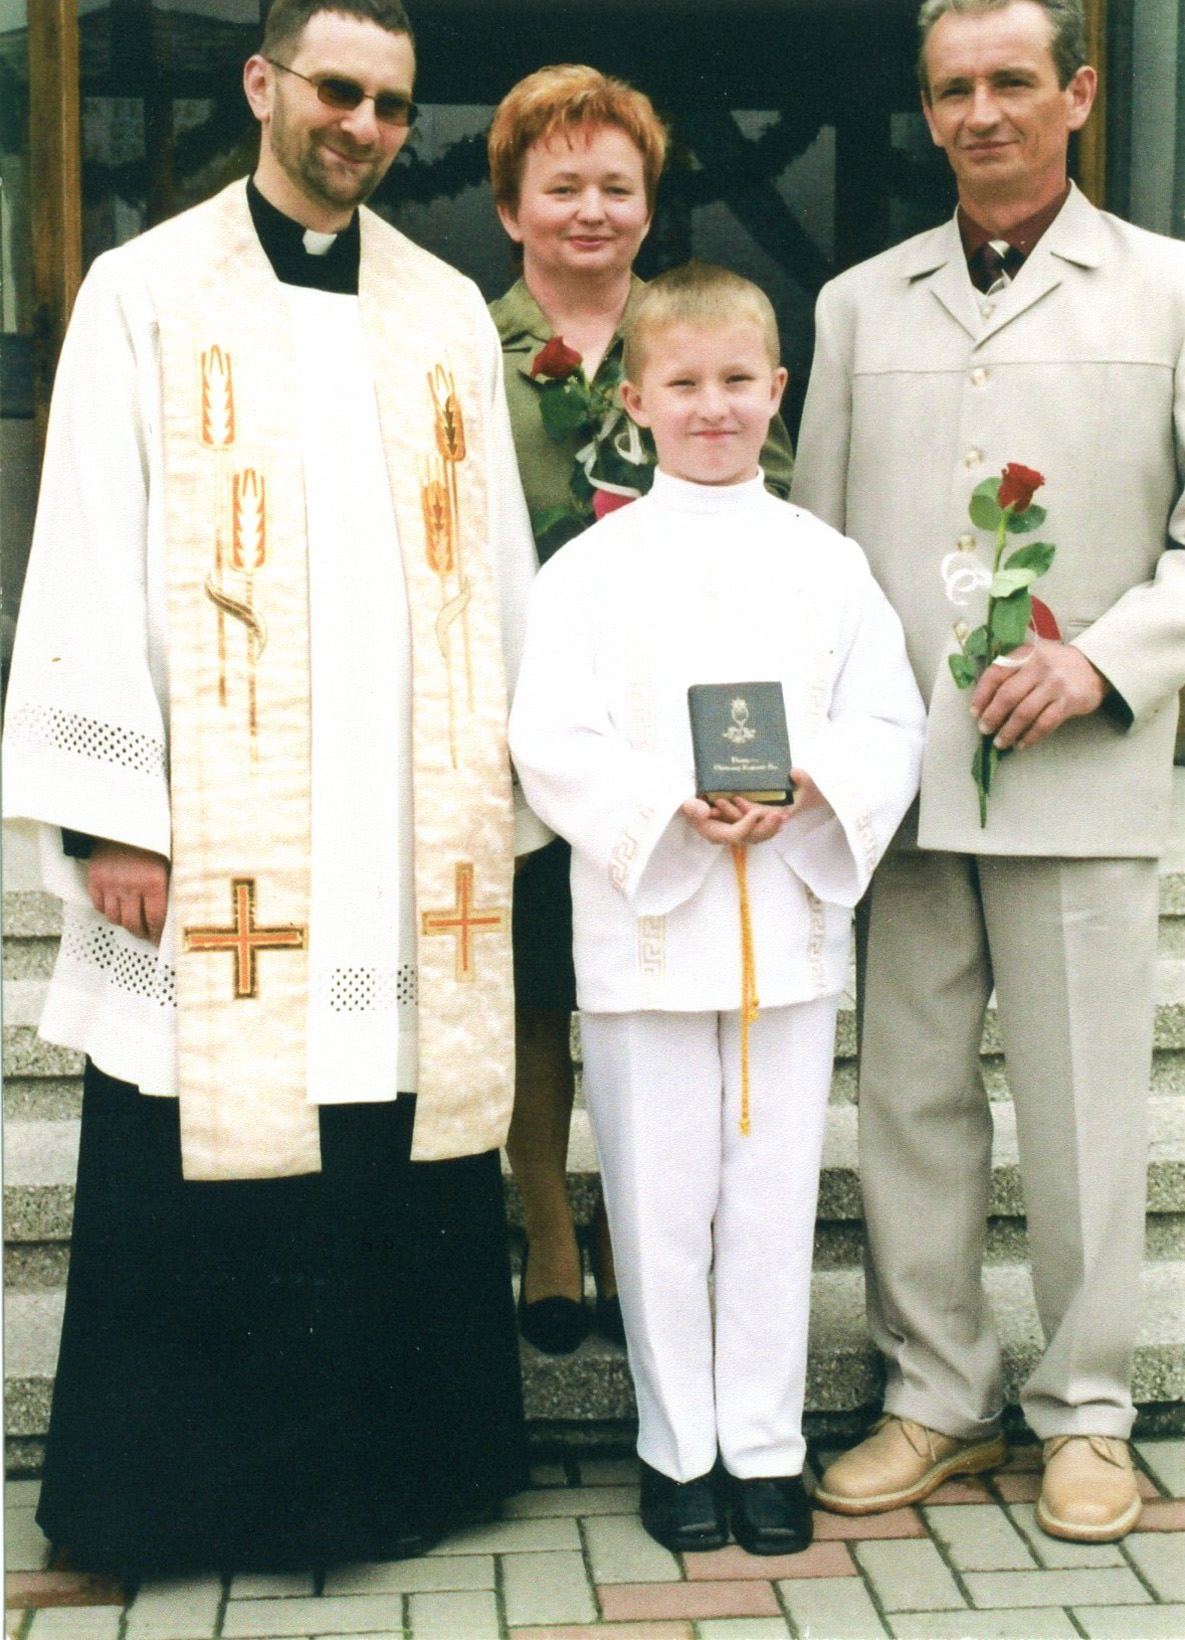
\includegraphics[width=0.3\textwidth]{photo/adam_kus_komunia.jpg}
\caption[Pierwsza Komunia św. Adama Kusia]{Pierwsza Komunia św. Adama Kusia, na zdj. Adaś z rodzicami i księdzem.}
\label{rys:adam_kus_komunia}
\end{center}
\end{figure}

\begin{sidewaysfigure}[!h]
\begin{center}
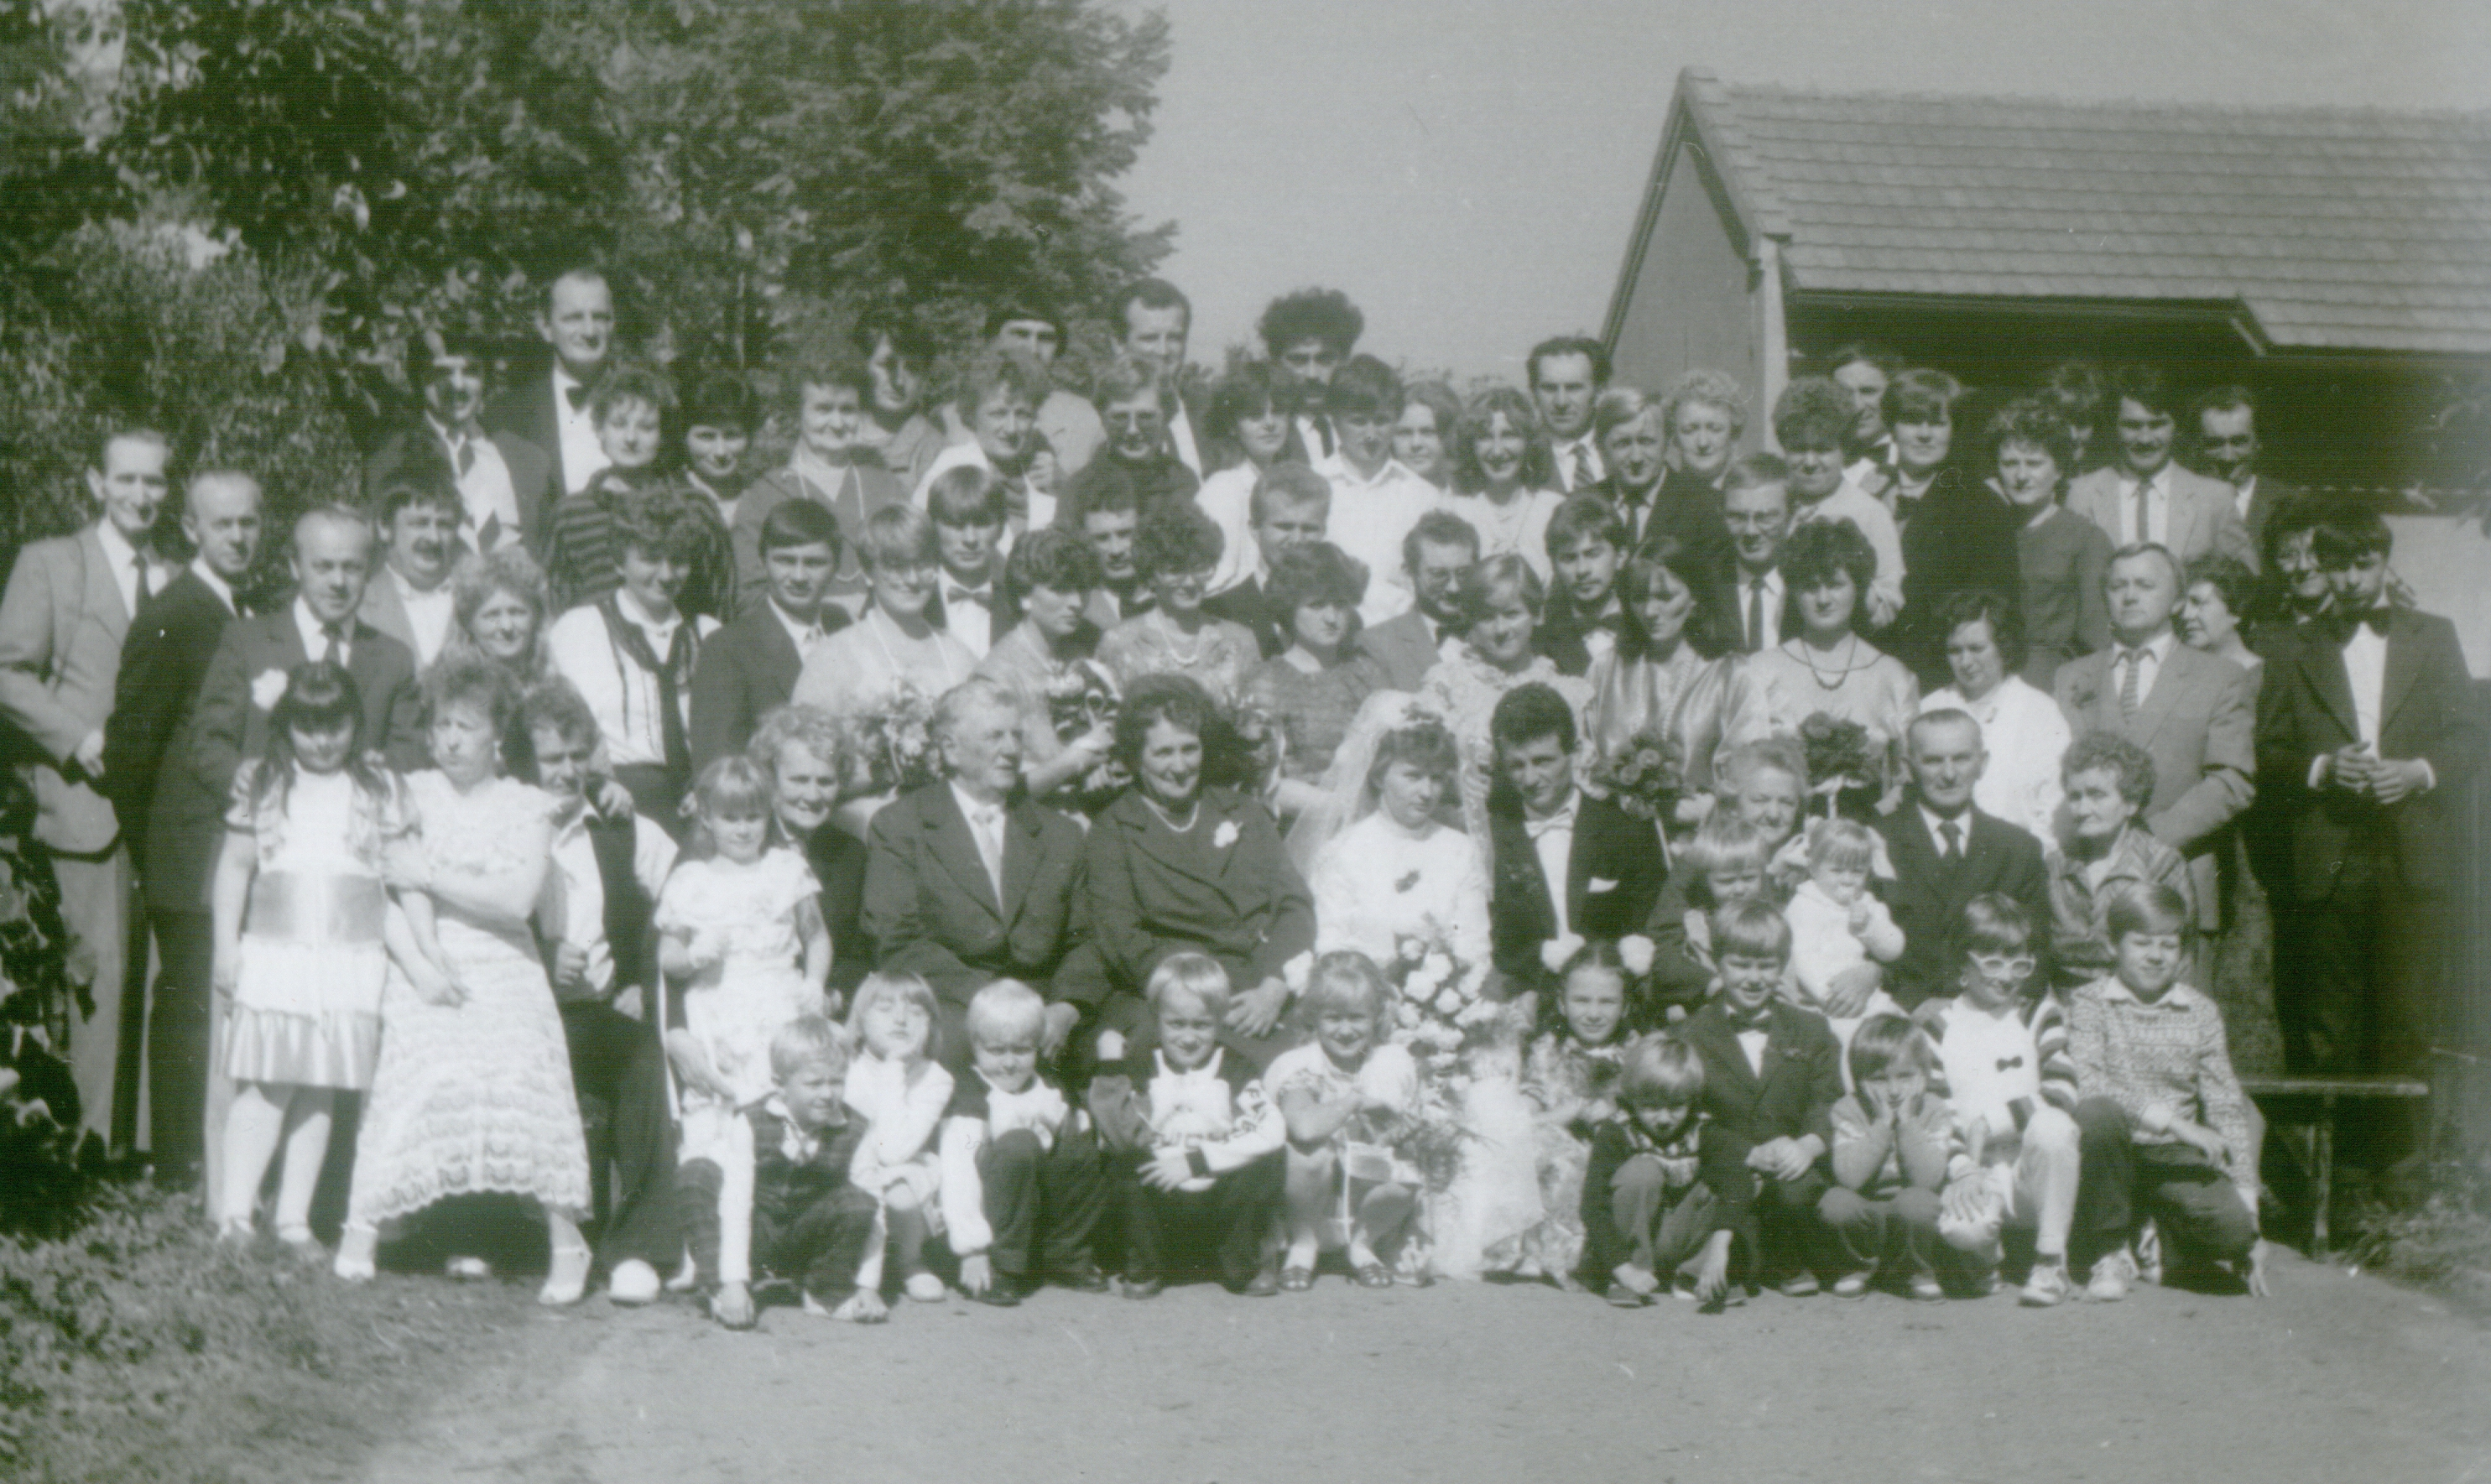
\includegraphics[height=149mm]{photo/bogdan_marysia_kus_slub_2.jpg}
\caption{Zdjęcie zbiorowe ze ślubu Bogdana i Marysi Kusiów}
\label{rys:bogdan_marysia_kus_slub_2}
\end{center}
\end{sidewaysfigure}

Utrzymują się z pracy na własnym gospodarstwie rolnym o pow. 14 ha, które wraz z dzierżawą ma powierzchnię 25 ha.

Obecny dom mieszkalny na Wieskach stoi w miejscu dawnego ogrodu.

Natomiast stary dom stał równolegle do dzisiejszego nowego chlewa, a na przedłużeniu obecnego starego chlewa. Stary dom był parterowy, murowany z cegły i otynkowany, połączony ze starym chlewem (jeszcze starszym od obecnego starego chlewa).

Dziadek Edward kupił ten dom wraz z polem i zabudowaniami gospodarskimi od Stanoska za pieniądze uzyskane od Wańczyka (wg relacji Ireny Lehman) lub od Kępy bądź Klamy (wg relacji Bogdana Kusia, który powziął tę informację od  Matki – Rozalii Kuś) za sprzedany dom w Łagiewnikach Wielkich przy ul. Szkolnej – vis a’ vis nowej szkoły. Tak więc stary dom, w którym przyszły na świat dzieci Edwarda i Eufemii wybudował prawdopodobnie Stanoszek.

Obecny -- nowy dom w latach 70’wybudowali Teodor i Rózia Kusiowie wraz ze swoimi dziećmi, dokąd się wprowadzili w 1972~r. Stary dom zburzyli Kusiowie w 1990~r.